\documentclass[xcolor=dvipsnames,10pt]{beamer}
% ********** Styl prezentacji **********
\mode<presentation>
{
%\usetheme{Frankfurt}
%\usetheme{Copenhagen}
\usetheme{Madrid}
 %\usetheme{lankton-keynote}
 %Copenhagen
}
%\usepackage{amsmath}
%\usepackage{amsthm}
%\usepackage{amsfonts}
\usepackage{color}
%\usepackage{listings}
%\lstset{language=C++}
%\usepackage{lscape} 
%\usepackage{float}
%\usepackage{graphicx}
\usepackage{caption}
\usepackage{subcaption}
%\usepackage{multimedia}
% common reference commands
\newcommand{\eqt}[1]{Eq.~(\ref{#1})}                     % equation
\newcommand{\fig}[1]{Fig.~\ref{#1}}                      % figure
\newcommand{\tbl}[1]{Table~\ref{#1}}                     % table
%\usepackage{movie15}
%\usepackage{hyperref}
%\usepackage{multimedia}
\usepackage[]{media9}
%\usepackage{filecontents,hyperref,listings}
\renewcommand{\div}{\vec{\nabla} \cdot}
\newcommand{\grad}{\vec{\nabla}}
%
%\setbeamertemplate{footline}[frame number]
%\title{Extension of the entropy viscosity method to low Mach regime and the seven equations model.}
%\title{Extension of the entropy viscosity method to low Mach regime and the seven equations model.}
%\author{Marc-Olivier Delchini}
%
\begin{document}
%
%\begin{frame}
%\maketitle
%\end{frame}
\begin{frame}
\centering
\large{Preliminary exam:}
\begin{center}
\begin{block}{\centering Extension of the entropy viscosity method to low Mach regime and multi-phase flows,}
\end{block}
\begin{center}
and
\end{center}
\begin{block}{\centering A Multi-Physics Example: application of the entropy viscosity method to the $1$-D grey Radiation-Hydrodynamic equations (RHD).}
\end{block}
\begin{center}
Marc-Olivier Delchini
\end{center}
\today \\

Co-chairs: J. Ragusa\footnote{Nuclear Engineering Department, Texas A\&M University.} and J.L. Guermond\footnote{Department of Mathematics, Texas A\&M University.}. \\
Committee members: J. Morel\footnotemark[1], Y. Hassan\footnotemark[1] and R. Berry\footnote{Idaho National Laboratory.}.
\end{center}
\end{frame}
%
\begin{frame}
	\frametitle{Outline:}
	\tableofcontents
\end{frame}
%************************************************
\section{Extension of the entropy viscosity method to low Mach regime and multi-phase flows.}
\begin{frame}
\begin{center}
\LARGE{Extension of the entropy viscosity method to low Mach regime and multi-phase flows.}
\end{center}
\end{frame}
%************************************************
\subsection{Computational method: background}
\begin{frame}{Background (1/2):}
\begin{block}{}
\begin{itemize}
\setlength{\itemsep}{10pt}
\item Hyperbolic system of equations $\rightarrow$ nuclear reactors, oil/gas models, aerospace, aeronautic, $\dots$ 
\item Single- and multi-phases flow. %: Euler equations, Homogeneous Equilibrium Model $(HEM)$, $5$ equations model (same pressure and velocity), $7$ equations model, $\dots$
\item Numerical methods required for stabilization purpose: shocks/discontinuities. 
\item Systems of equations describing the physics must be well-posed $\rightarrow$ real eigenvalues.
\item {\color{red}Entropy condition:} ensures convergence of the numerical solution to the physical solution.
\end{itemize}
\end{block}
\end{frame}
%************************************************
\begin{frame}{Background (2/2):}
\begin{block}{Numerical methods for continuous and discontinuous schemes:}
\begin{itemize}
\setlength{\itemsep}{10pt}
\item Approximate Riemann solvers \cite{Toro}: HLL, HLLC, Roe scheme, $\cdots$
\item Flux limiters \cite{FluxLimiter1, FluxLimiter2, FluxLimiter3, FluxLimiter4}.
\item Lapidus viscosity \cite{Lapidus_paper, Lapidus_book, LMP}, Pressure-based viscosity \cite{PBV_book}. 
\item C-method \cite{Reisner}.
\item Streamline Upwind Petrov-Galerkin (SUPG) \cite{SUPG}.
\item Entropy viscosity method \cite{jlg1, jlg2, jlg3}.
\end{itemize}
\end{block}
\begin{block}{}
These numerical methods are mainly used with high-order explicit temporal integrators.
\end{block}
\end{frame}
%************************************************
\begin{frame}{Low Mach regime:}
\begin{block}{}
{\color{red}The numerical methods developed to resolve shocks for supersonic flows are usually ill-scaled in the low Mach regime \cite{LowMach1, LowMach2, LowMach3}.} 
\begin{itemize}
\item The dissipative terms become dominant and change the nature of the equations.
\item A fix is often required in the low Mach regime in order to yield the correct behavior $\rightarrow$ add enough viscosity to stabilize the scheme but not too much so that the physical solution is not altered. 
\item Example with Roe scheme \cite{Roe}: a fix was designed in order to obtain the correct asymptotic behavior in the low Mach regime.
\begin{equation}
\mathbf{F}(\mathbf{U}) = (1-M) \cdot \mathbf{F}_{\text{Low Mach}}(\mathbf{U}) + M \cdot \mathbf{F}_{Roe}(\mathbf{U}) \nonumber
\end{equation}
\item Example of scaling analysis with artificial dissipative terms: upwind scheme.
\begin{equation}
\partial_{t} \rho + \div \left( \rho \vec{u} \right) = \frac{1}{2}\left( 1 + \frac{1}{M^*} \right)  \div \left(\kappa \grad \rho \right) \nonumber
\end{equation}
\end{itemize}
\end{block}
\end{frame}
%************************************************
%\subsection{RELAP-7: reactor safety analysis code.}
%\begin{frame}{RELAP-7: reactor safety analysis code.}
%\begin{block}{What is RELAP-7?}
%\begin{itemize}
%\setlength{\itemsep}{15pt}
%\item Developed by Idaho National Laboratory (INL). 
%\item $1$-D reactor analysis system.
%\item Based on the MOOSE \cite{Moose} framework (C++): fully implicit code.
%\item Safety applications for PWR, BWR and gas reactors.
%\item Solve compressible system of equations using conservative variables $(\rho, \rho \vec{u}, \rho E)$.
%\end{itemize}
%\end{block}
%\end{frame}
%************************************************
\begin{frame}
\begin{block}{Fluid solver requirements:}
\begin{enumerate}
\setlength{\itemsep}{1pt}
\item Compressible single and two-phase flow equations.
\item Being able to resolve shocks: numerical method.
\item Valid for any equation of state of type $P = eos(\rho, e)$.
\item Valid for a wide range of Mach numbers: compressible and incompressible flows.
\item Account for source terms: wall friction, wall heat source, gravity force, $\dots$
\item Use \emph{implicit} temporal integrators: Backward Euler and BDF2.
\end{enumerate}
\end{block}
\begin{block}{The entropy viscosity method, a good candidate?}
\begin{itemize}
\setlength{\itemsep}{1pt}
\item 1 and 2 are met by the entropy viscosity method ONLY for single-phase flow.
\item 3: there exists a theoretical proof that states the method can be applied to any EOS with a convex entropy function.
\item 4, 5 and 6 are investigated here.
\end{itemize}
\end{block}
\end{frame}
%************************************************
%\subsection{The entropy viscosity method.}
%\begin{frame}{The entropy function:}
%For a given hyperbolic system of equations: $\partial_t \mathbf{U} + \div \mathbf{F} \left( \mathbf{U} \right) = 0$
%\begin{block}{Definition of the physical entropy (ref):}
%An entropy is a function that is positive and increases with time: 
%\end{block}
%\begin{block}{Entropy inequality (ref):}
%\begin{equation}
%\partial_t \mathbf{U} + \div \mathbf{F} \left( \mathbf{U} \right) = 0 \Rightarrow \partial_t s + \div \Phi (s)  \geq 0 \nonumber
%\end{equation}
%\end{block}
%\begin{block}{Example: multi-D Euler equations \cite{Toro}}
%\begin{equation}
%\partial_t s(\rho,e) + \vec{u} \cdot \grad s(\rho,e) \geq 0 \nonumber
%\end{equation}
%\end{block}
%\end{frame}
%************************************************
\begin{frame}{The entropy viscosity method \cite{jlg}:}
It is based on the entropy production that occurs in shock and the entropy minimum principle.
\begin{block}{}
\begin{itemize}
\setlength{\itemsep}{10pt}
\item Add artificial dissipative terms consistent with the entropy minimum principle.
\item Define a local and smooth viscosity coefficient function of the grid size.
\item The viscosity coefficient is defined proportional to the entropy production.
\item The entropy production is locally computed by evaluating the entropy residual:
\begin{equation}
D_e(\vec{r},t) = \partial_t s + \vec{u} \cdot \grad s \geq 0 \nonumber
\end{equation}
\centering
(Euler equations)
\end{itemize}
\end{block}
\end{frame}
%************************************************
\begin{frame}{Application to the multi-D Euler equations \cite{valentin}:}
\begin{block}{The multi-D Euler Equations: \cite{Toro}}
\begin{eqnarray}
\left\{
\begin{array}{llll}
\partial_t \rho + \div \left(\rho \vec{u} \right) = {\color{red}\div \left(\kappa \grad \rho \right)}  \\
\partial_t \left(\rho \vec{u} \right) + \div \left(\rho \vec{u} \otimes \vec{u} \right) + \grad P = {\color{red}\div\left[ \left( \mu \rho \grad^s \vec{u} + \vec{u} \otimes \left( \kappa \grad \rho \right) \right)\right]}   \nonumber\\
\partial_t \left(\rho E \right) + \div \left[\vec{u}(\rho E + P)\right] = {\color{red}\div\left[ \left( \kappa \grad (\rho e) + \frac{||\vec{u}||^2}{2} \kappa \grad \rho + \mu \rho \vec{u} \cdot \grad^s \vec{u} \right)\right]} \\
P = eos(\rho, e) 
\end{array}
\right.
\end{eqnarray}
\end{block}
\begin{block}{Definition of the local viscosity coefficients $\mu$ and $\kappa$: ($\mu = \kappa$)}
\begin{eqnarray}
\left\{
\begin{array}{lll}
\mu(\vec{r},t) = \min(\mu_e(\vec{r},t), \mu_{max}(\vec{r},t)) \\
\mu_e(\vec{r},t) = h^2 \frac{\max(D_e(\vec{r},t), J)}{|| s(\vec{r},t) - \bar{s}(t) ||_{\infty}}\\
\mu_{max}(\vec{r},t) =  \frac{h}{2} \left( ||\vec{u}|| + c \right) \\
D_e(\vec{r},t) = \partial_t s + \vec{u}  \cdot\div \left( s \right) \geq 0 \text{ with } s\left( \rho, e \right) \geq 0
\end{array}
\right.
\nonumber
\end{eqnarray}
\end{block}
\end{frame}
%************************************************
\subsection{The multi-D Euler equations (with variable area).}
\begin{frame}{The multi-D Euler equations (with variable area) \cite{Toro}:}
\begin{block}{The multi-D Euler Equations (with variable area):}
\begin{eqnarray}
\left\{
\begin{array}{llll}
\partial_t (\rho A) + \div \left(\rho \vec{u} A\right) = 0  \\
\partial_t \left(\rho \vec{u}A\right) + \div \left(A\rho \vec{u} \otimes \vec{u} \right) + \grad (AP) = \underbrace{P \grad A}_{\text{extra term}} \\
\partial_t \left(\rho E A\right) + \div \left[\vec{u}A(\rho E + P)\right] = 0 \\
P = eos(\rho, e) 
\end{array}
\right.
\nonumber
\end{eqnarray}
$\rho$ is the density, $P$ the pressure, $E$ the specific total energy, $\vec{u}$ the velocity, $e$ the internal energy, and $A$ the area.
\end{block}
\begin{block}{A few remarks:}
\begin{itemize}
\setlength{\itemsep}{1pt}
\item The area $A$ is assumed to be spatially dependent only: $A(\vec{r})$.
\item For the purpose of this proposal, $A(\vec{r})$ is assumed to be smooth: $1$-D nozzle.
\item The eigenvalues are unchanged.
\end{itemize}
\end{block}
\end{frame}
%************************************************
\subsubsection{Proposal.}
\begin{frame}
\begin{block}{Proposal (1/3): theoretical approach.}
\begin{enumerate}
\setlength{\itemsep}{2pt}
\item Derive the dissipative terms using the entropy minimum principle: this step is straightforward with help of \cite{jlg}.
\item Investigate the low Mach regime $\rightarrow$ the entropy residual will be recast under the following form:
\begin{equation}
D_e(\vec{r},t) = \partial_t s + \vec{u} \cdot \grad s = \frac{s_e}{P_e} \underbrace{\left( \frac{d P}{dt} - c^2 \frac{d \rho}{dt} \right)}_{\tilde{D}_e(\vec{r},t)} \nonumber
\end{equation}
\begin{itemize}
\item $\tilde{D}_e(\vec{r},t)$ is an alternative way of computing the local entropy production.
\item The viscosity coefficient will be set proportional to $\tilde{D}_e(\vec{r},t)$ (instead of $D_e(\vec{r},t)$):
\begin{equation}
\mu_e(\vec{r},t) = h^2 \frac{\tilde{D}_e(\vec{r},t)}{f(P)} \nonumber
\end{equation}
\item This new expression offers more diversity in the choice of the normalization parameter $f(P)$: $P$, $\rho c^2$, $\rho c ||\vec{u} ||$ or  $\rho ||\vec{u}||^2$.
\item $f(P)$ will be determined by doing a low Mach asymptotic study of the multi-D Euler equations.
\end{itemize}
\end{enumerate}
\end{block}
\end{frame}
%************************************************
\begin{frame}
\begin{block}{Proposal (2/3): perform $1$-D tests.}
\begin{enumerate}
\setcounter{enumi}{2}
\item Sod shock tubes \cite{Toro} with Ideal Gas equation of state \cite{IGEOS}:
\begin{center}
$P = (\gamma-1) \rho e$
\end{center}
\item $1$-D nozzle with Stiffened Gas equation of state \cite{SGEOS}: vapor phase (supersonic flow) and liquid phase (subsonic flow) {\color{magenta}NEW}.
\begin{center}
$P = (\gamma-1) \rho (e-q) - \gamma P_{\infty}$
\end{center}
There is an analytical solution for steady-state.
\item Tait equation of state \cite{ShockTEOS} (?) {\color{magenta}NEW}
\begin{center}
$P = P_0 \left( 1-\frac{\rho}{\rho_0} \right)^{\gamma-1}$
\end{center}
\item Investigate the effect of source terms on the method. Tests will be performed for a $1$-D core channel of a PWR using RELAP-$7$ code {\color{magenta}NEW}. \\
$\rightarrow$ derive the entropy residual with the source terms.
\end{enumerate}
\end{block}
\end{frame}
\begin{frame}
%************************************************
\begin{block}{Proposal (3/3): perform $2$-D tests.}
\begin{enumerate}
\setcounter{enumi}{4}
\setlength{\itemsep}{10pt}
\item Perform $2$-D tests for supersonic flows: 
\begin{itemize}
\setlength{\itemsep}{10pt}
\item Forward facing step \cite{Mach3Step}.
\item Riemann problem $12$ \cite{Riemann12}.
\item Sedov test \cite{Toro}.
\item Compression and decompression corner \cite{CompressionCorner}.
\end{itemize}
\item Perform $2$-D tests for subsonic flow: hump (no analytical solution) and cylinder (analytical solution). {\color{magenta}NEW}
\begin{itemize}
\setlength{\itemsep}{10pt}
\item Hump \cite{Hump}.
\item Cylinder \cite{LowMach3}.
\end{itemize}
\end{enumerate}
\end{block}
\end{frame}
%************************************************
\subsubsection{Preliminary numerical results.}
\begin{frame}{$1$-D numerical results: Leblanc shock tube \cite{Leblanc}.}
\begin{figure}[H]
        \centering
        \begin{subfigure}[b]{0.4\textwidth}
                \centering
                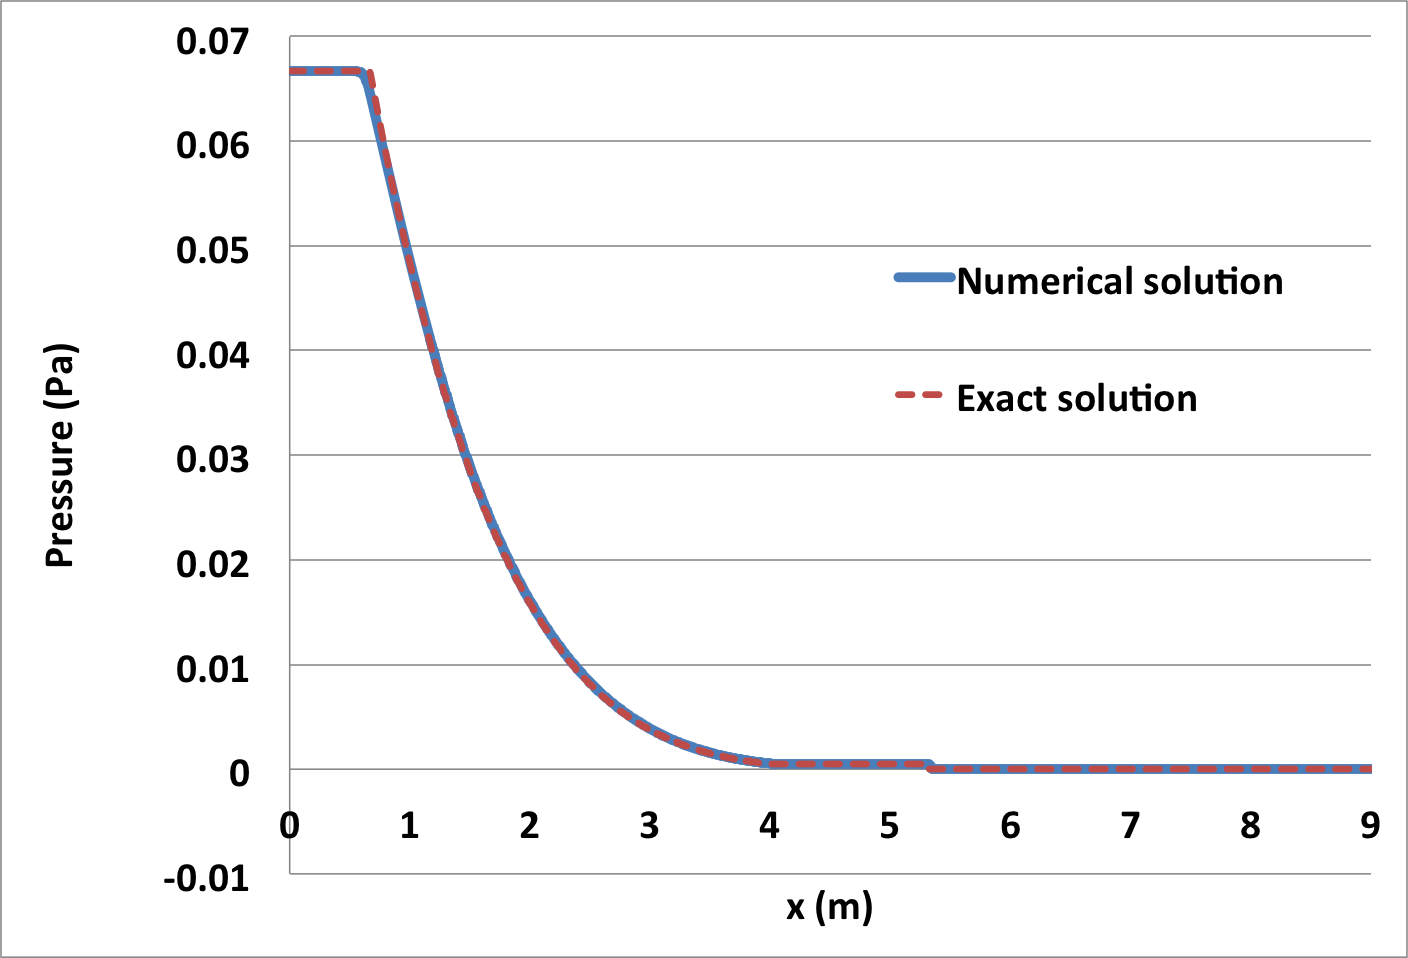
\includegraphics[width=\textwidth]{Leblanc_pressure.png}
%                \caption{Pressure}
        \end{subfigure}%
        ~ %add desired spacing between images, e. g. ~, \quad, \qquad etc. 
          %(or a blank line to force the subfigure onto a new line)
        \begin{subfigure}[b]{0.4\textwidth}
                \centering
                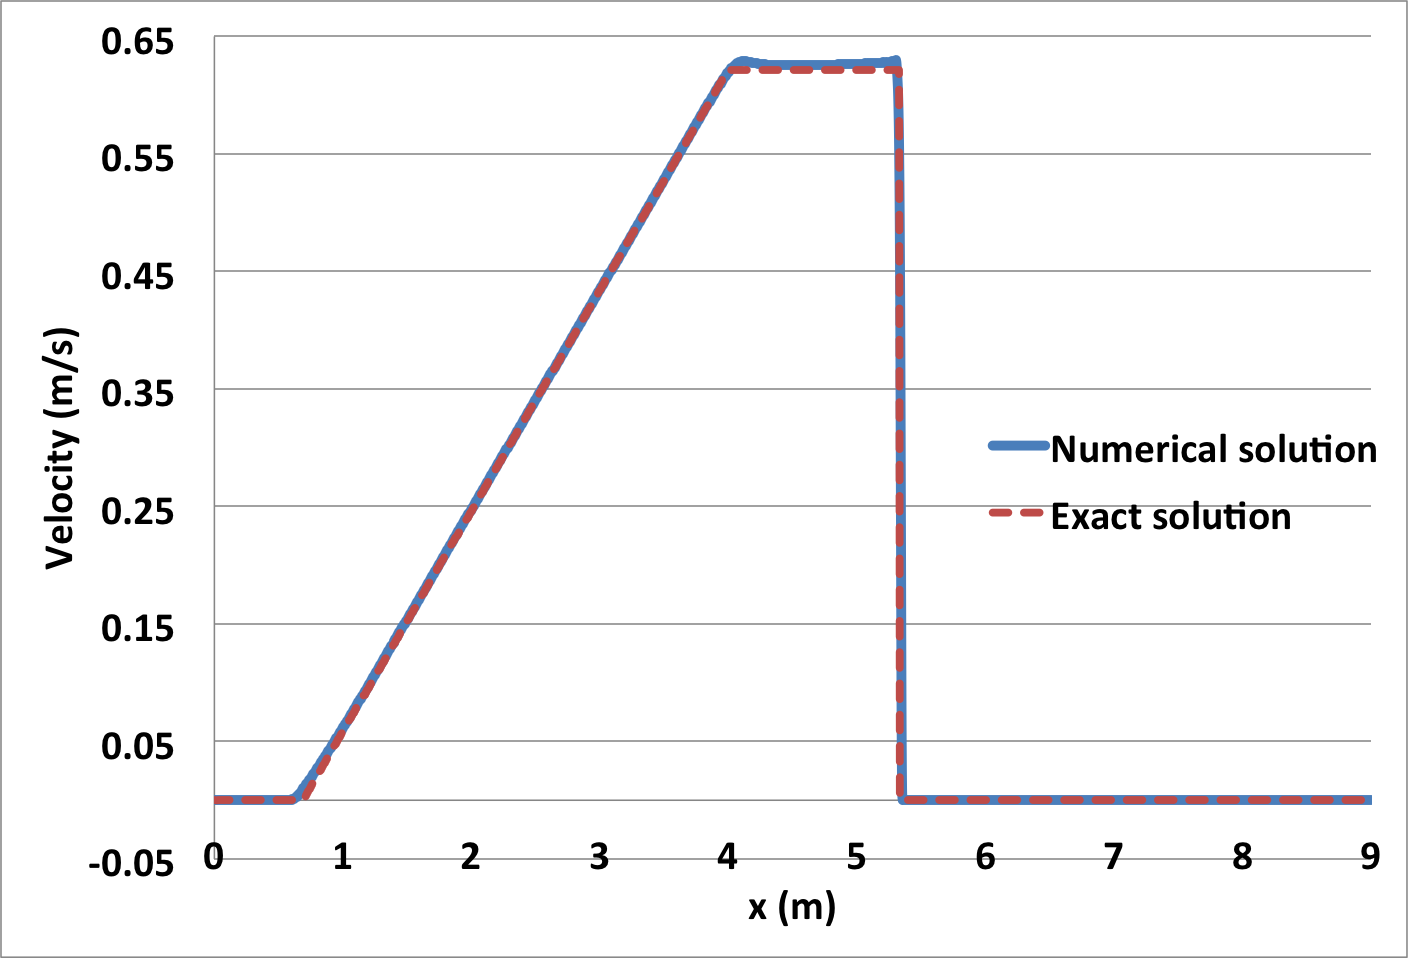
\includegraphics[width=\textwidth]{Leblanc_velocity.png}
%                \caption{Velocity.}
        \end{subfigure}
         %add desired spacing between images, e. g. ~, \quad, \qquad etc. 
          %(or a blank line to force the subfigure onto a new line)
        \begin{subfigure}[b]{0.4\textwidth}
                \centering
                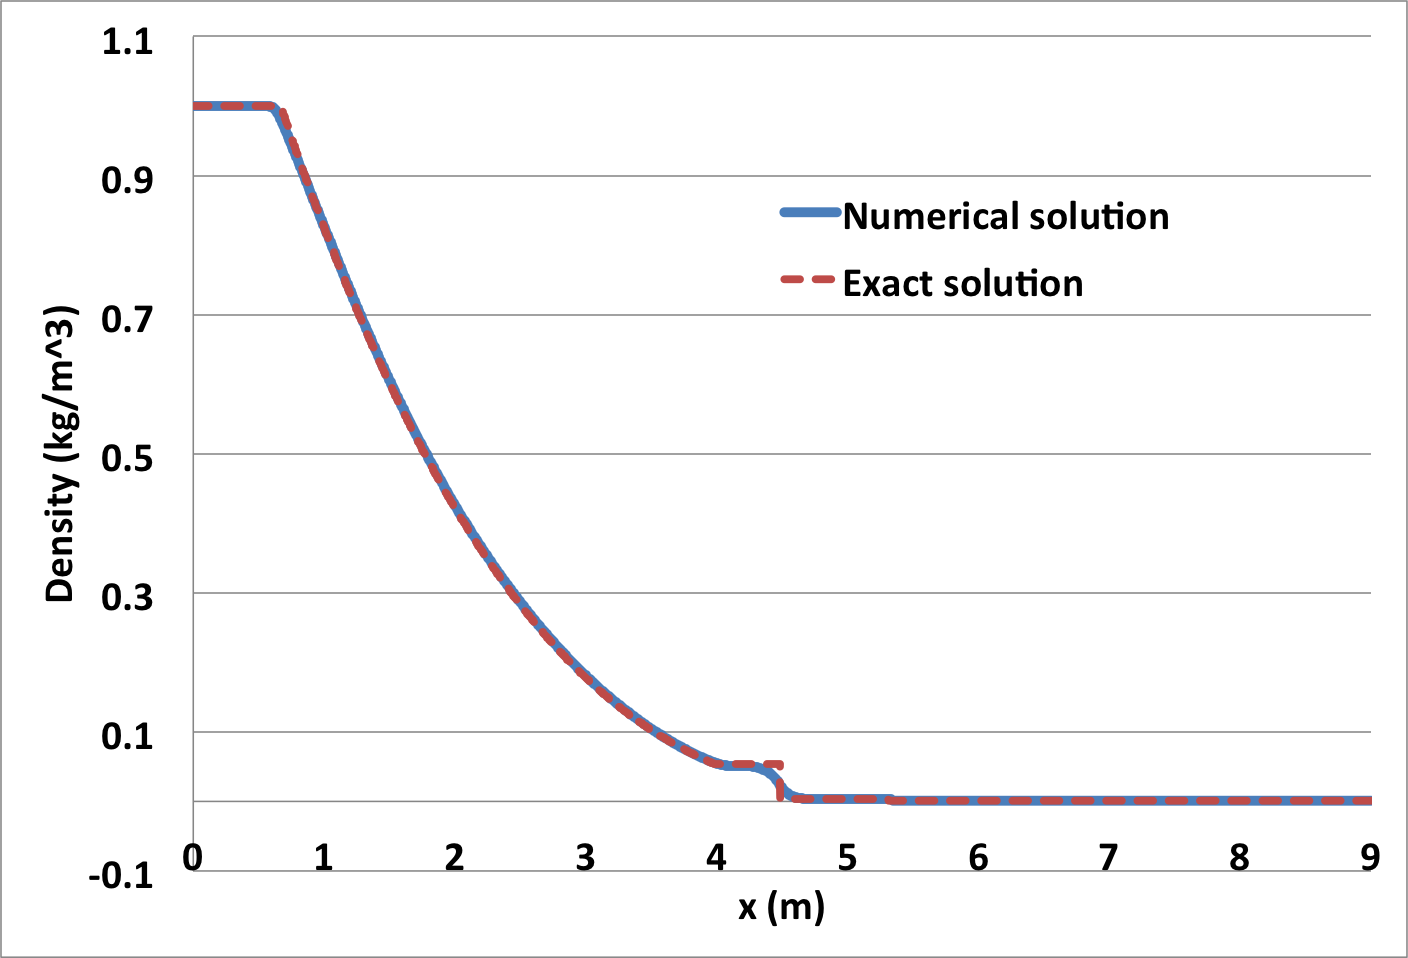
\includegraphics[width=\textwidth]{Leblanc_density.png}
%                \caption{Density.}
        \end{subfigure}
         \begin{subfigure}[b]{0.4\textwidth}
                \centering
                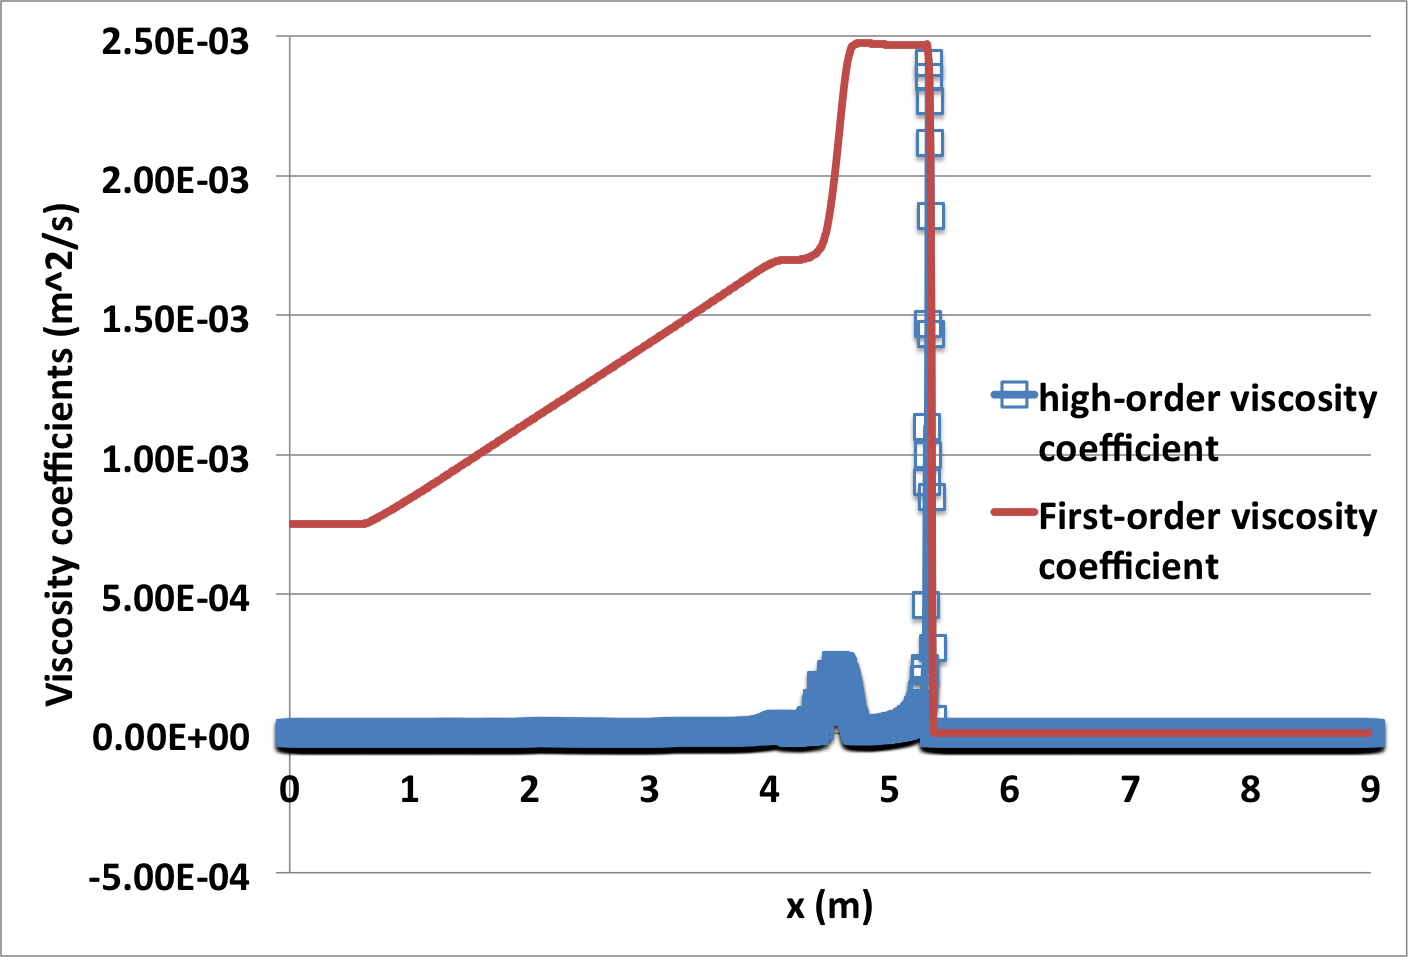
\includegraphics[width=\textwidth]{Leblanc_viscosity.png}
%                \caption{Viscosity coefficients.}
        \end{subfigure}
        \caption{Numerical solution at $t=4.s$ with $2000$ cells, linear polynomials and BDF2.}
\end{figure}
\end{frame}
%************************************************
\begin{frame}{$2$-D numerical results: compression corner ($M=2.5$).}
\begin{center}
  \begin{columns}
    \column{.5\textwidth}
       \includemedia[addresource=compression_corner.mp4, activate=pageopen, deactivate=pageclose, width=6.5cm, height=5cm, flashvars={source=compression_corner.mp4 & autoPlay=true & loop=true }]{}{VPlayer.swf}
    \column{.5\textwidth}
      \includemedia[addresource=compression_corner_viscosity.mp4, activate=pageopen, deactivate=pageclose, width=6.5cm, height=5cm, flashvars={source=compression_corner_viscosity.mp4 & autoPlay=true & loop=true }]{}{VPlayer.swf}
  \end{columns}
\end{center}
\end{frame}
%************************************************
\subsubsection{Conclusions: the multi-D Euler equations.}
\begin{frame}{Conclusions: the multi-D Euler equations.}
\begin{block}{What we have done so far:}
\begin{itemize}
\setlength{\itemsep}{20pt}
\item Derived a definition for the viscosity coefficient that is consistent for supersonic and subsonic flows (hump).
\item Tested the new definition of the viscosity coefficients with $1$- and $2$-D tests.
\item Investigated the effect of the source terms on the method and performed a test on a $1$-D PWR core channel (RELAP-7).
\end{itemize}
\end{block}
\begin{block}{What is left to do:}
\begin{itemize}
\item Remains to test the method for a subsonic flow around a cylinder: good test since an analytical steady-state solution is available (appendix).
\end{itemize}
\end{block}
\end{frame}
%************************************************
\subsection{The multi-D seven-equation model (with variable area).}
\begin{frame}{The multi-D seven-equation model (with variable area) \cite{SEM}:}
\begin{block}{The model:}
\begin{itemize}
\setlength{\itemsep}{10pt}
\item Each phase obeys the single-phase Euler equations: two continuity equations, two momentum equations and two energy equations.
\item Seventh equation: void fraction equation $\rightarrow$ an internal boundary condition between the two phases at the interface.
\item Exchange terms between phases: relaxation terms. These terms were derived using \emph{rational thermodynamic} \cite{RatTherm} $\rightarrow$ consistent with the entropy minimum principle.
\item {\color{red}The system of equations is well-posed, it has 7 real eigenvalues.}
\item The seven-equation model degenerates to single-phase Euler equations when one phase disappears.
\end{itemize}
\end{block}
\end{frame}
%************************************************
\begin{frame}{The multi-D seven-equation model (with variable area) \cite{SEM}:}
We consider two phases ${j,k}$. Phase $k$ obeys the following system of equations:
\begin{equation}
\left\{
\begin{array}{lcll}
\partial_t \left( \alpha_k  A\right) &+& \vec{u}_I A \grad \alpha_k = {\color{blue}A \mu_{rel} \left( P_k - P_j \right)}& \nonumber \\
\partial_t \left( \alpha_k \rho_k A \right) &+& \div \left( \alpha_k \rho_k \vec{u}_k A \right) = 0& \nonumber \\
\partial_t \left( \alpha_k \rho_k \vec{u}_k A \right) &+& \div \left[ \alpha_k A \left( \rho_k \vec{u}_k\otimes \vec{u}_k \right) \right]  + \grad(\alpha_k A P_k) =  \nonumber \\
&&\alpha_k P_k \grad A +  P_I A \grad \alpha_k +  {\color{blue}A \lambda_{rel} \left( \vec{u}_j - \vec{u}_k \right)} &\nonumber \\
\partial_t \left( \alpha_k \rho_k E_k A \right) &+& \div \left[ \alpha_k A \vec{u}_j \left( \rho_k E_k + P_k \right) \right] =& \\
&&P_I \vec{u}_I A \grad \alpha_k - {\color{blue}\mu_{rel} \bar{P_I} \left( P_k-P_j \right)} +{\color{blue}\bar{\vec{u}}_kA \lambda_{rel} \left( \vec{u}_j - \vec{u}_k \right)}& \nonumber
\end{array}
\right.
\end{equation}
\begin{equation}
\left\{
\begin{array}{l}
P_I = \bar{P_I} - \frac{\grad \alpha_k}{|\grad \alpha_k|} \frac{Z_k Z_j}{Z_k + Z_j} \cdot \left( \vec{u}_k-\vec{u}_j \right) \\
\bar{P_I} = \frac{Z_k P_j + Z_j P_k}{Z_k + Z_j} \\
\vec{u}_I = \bar{\vec{u}}_I - \frac{\grad \alpha_k}{|\grad \alpha_k|} \frac{P_k - P_j}{Z_k + Z_j} \\
\bar{\vec{u}}_I = \frac{Z_k \vec{u} _k + Z_j \vec{u}_j}{Z_k + Z_j} \\
\end{array}
\right.
\nonumber
\text{ and }
\left\{
\begin{array}{l}
\mu_{rel} = \frac{A_{int}}{Z_k+Z_j} \\
\lambda_{rel} = \frac{\mu_{rel}}{2} Z_k Z_j \\
A_{int} = 6.25 \cdot A_{int,max} \cdot \alpha_k \left( 1-\alpha_k \right)^2
\end{array}
\right.
\end{equation}
\end{frame}
%************************************************
\subsubsection{Proposal.}
\begin{frame}{}
\begin{block}{Proposal: theoretical approach (1/3) {\color{magenta}NEW}.}
\begin{enumerate}
\setlength{\itemsep}{10pt}
\item Derive the dissipative terms using the entropy minimum principle. For continuity, momentum and energy equations, the dissipative terms should be similar to what is obtained for Euler equations. The dissipative term of the void-fraction equation should be of the form $\div \left( \beta \grad \alpha_k \right)$.
\item Define the viscosity coefficients: $\mu$, $\kappa$ and $\beta$.
\item Investigate the low Mach regime $\rightarrow$ results from Euler equations hold. What about $\beta$?
\end{enumerate}
\end{block}
\begin{block}{Proposal: $1$-D tests (2/3) {\color{magenta}NEW}.}
\begin{enumerate}
\setlength{\itemsep}{5pt}
\setcounter{enumi}{4}
\item $1$-D nozzle with Stiffened Gas equation of state \cite{SEM}.
\end{enumerate}
\end{block}
\begin{block}{Proposal: $2$-D tests (3/3) {\color{magenta}NEW}.}
\begin{enumerate}
\setlength{\itemsep}{5pt}
\setcounter{enumi}{5}
\item Vapor + liquid shock tubes.
\end{enumerate}
\end{block}
\end{frame}
%************************************************
\subsubsection{Preliminary numerical results.}
\begin{frame}{$1$-D numerical results: nozzle.}
\centering
$\mu_{rel}$ and $\lambda_{rel}$ $\to \infty$
\begin{figure}[H]
        \centering
        \begin{subfigure}[b]{0.4\textwidth}
                \centering
                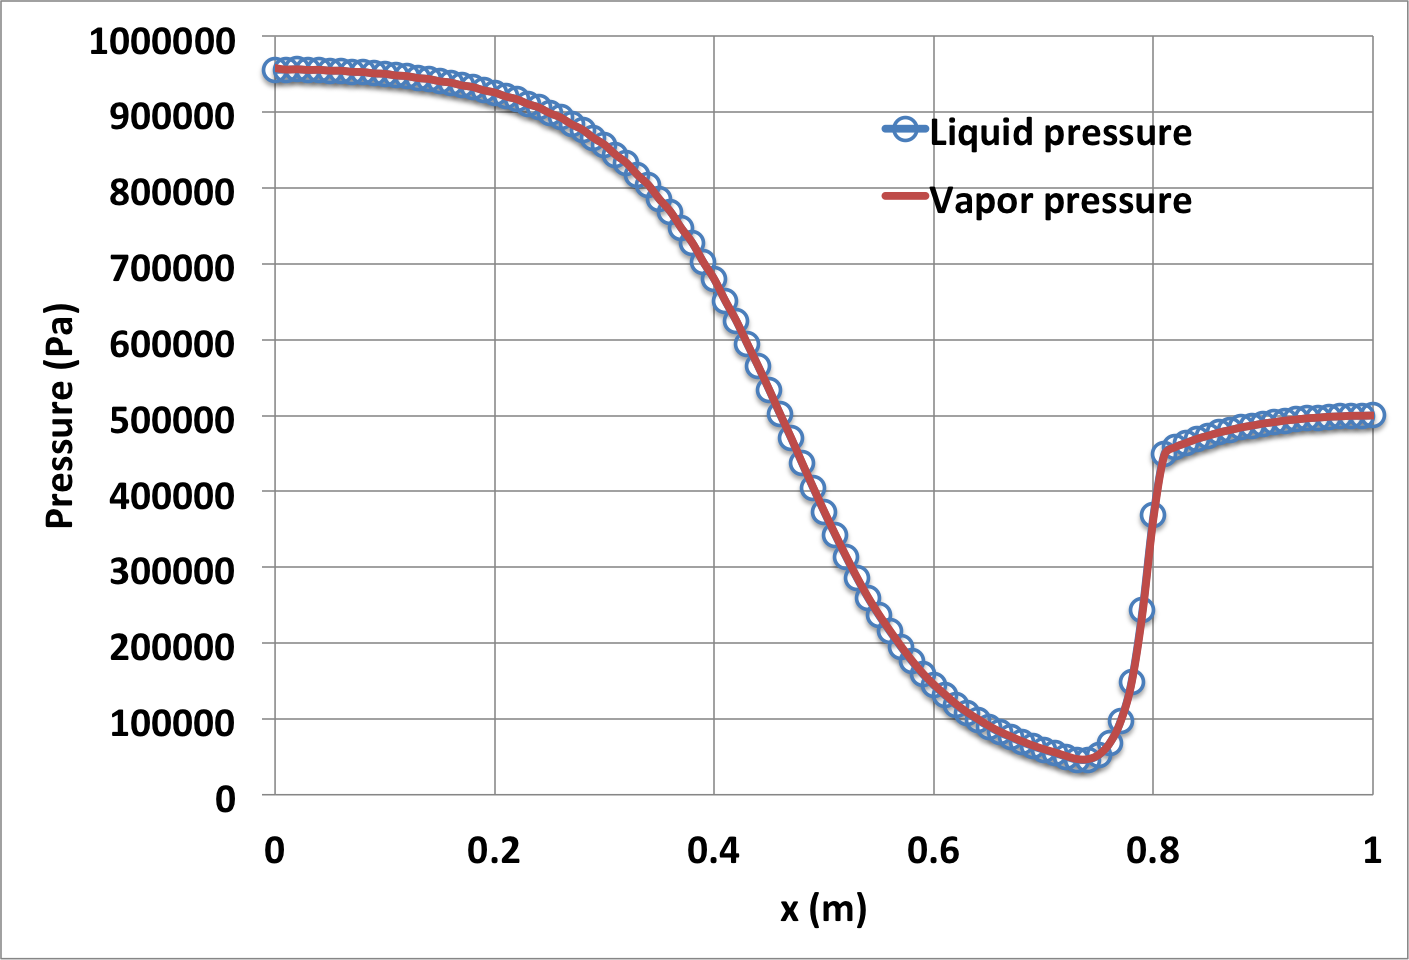
\includegraphics[width=\textwidth]{Sevan_pressure.png}
%                \caption{Pressure}
        \end{subfigure}%
        ~ %add desired spacing between images, e. g. ~, \quad, \qquad etc. 
          %(or a blank line to force the subfigure onto a new line)
        \begin{subfigure}[b]{0.4\textwidth}
                \centering
                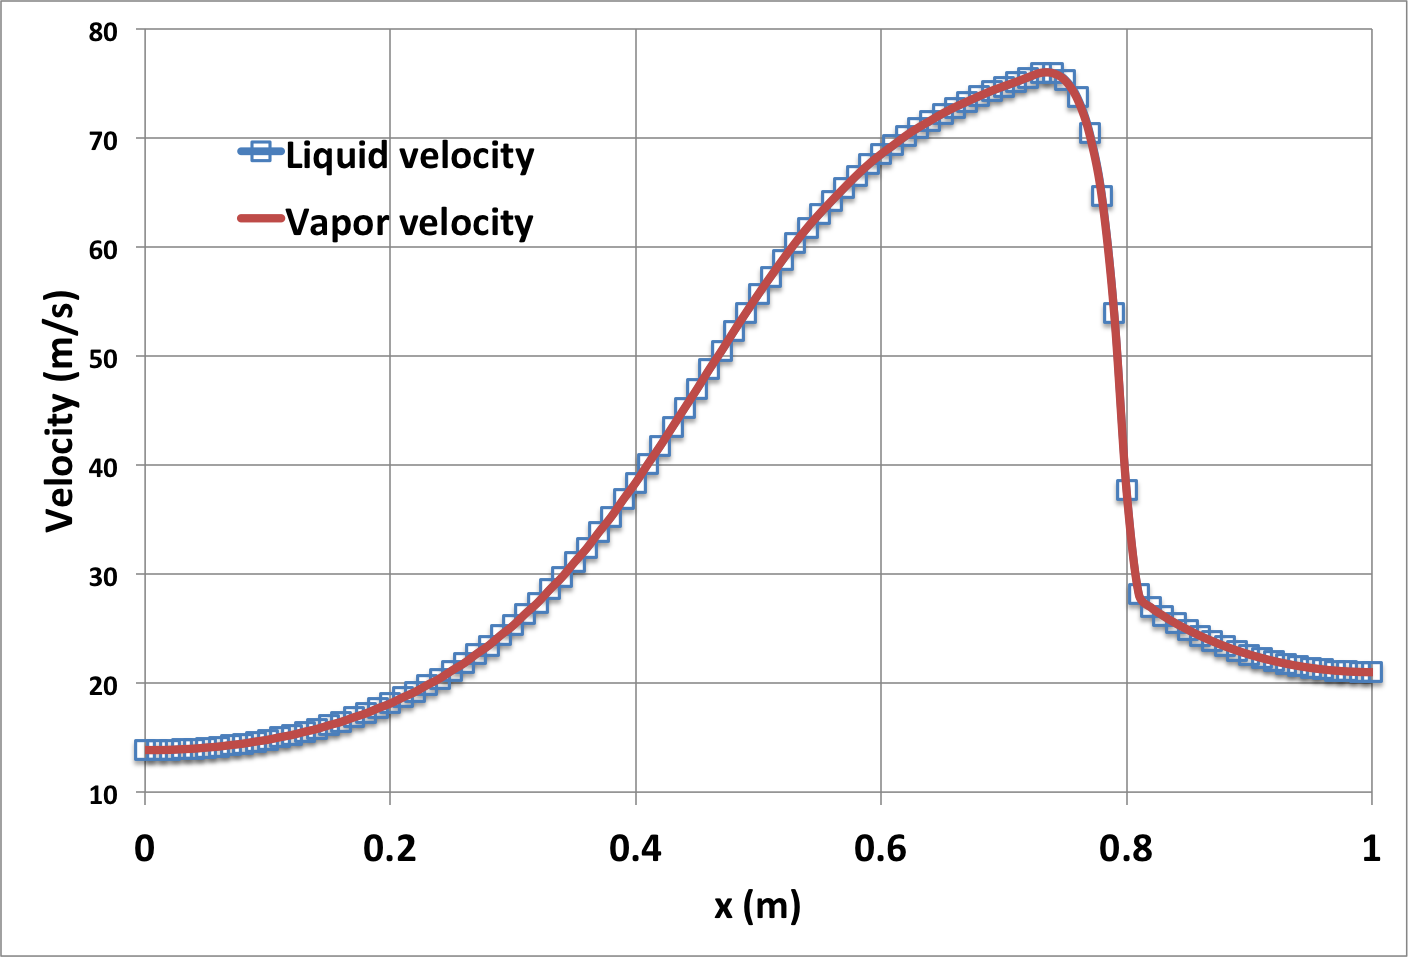
\includegraphics[width=\textwidth]{Sevan_velocity.png}
%                \caption{Velocity.}
        \end{subfigure}
         %add desired spacing between images, e. g. ~, \quad, \qquad etc. 
          %(or a blank line to force the subfigure onto a new line)
        \begin{subfigure}[b]{0.4\textwidth}
                \centering
                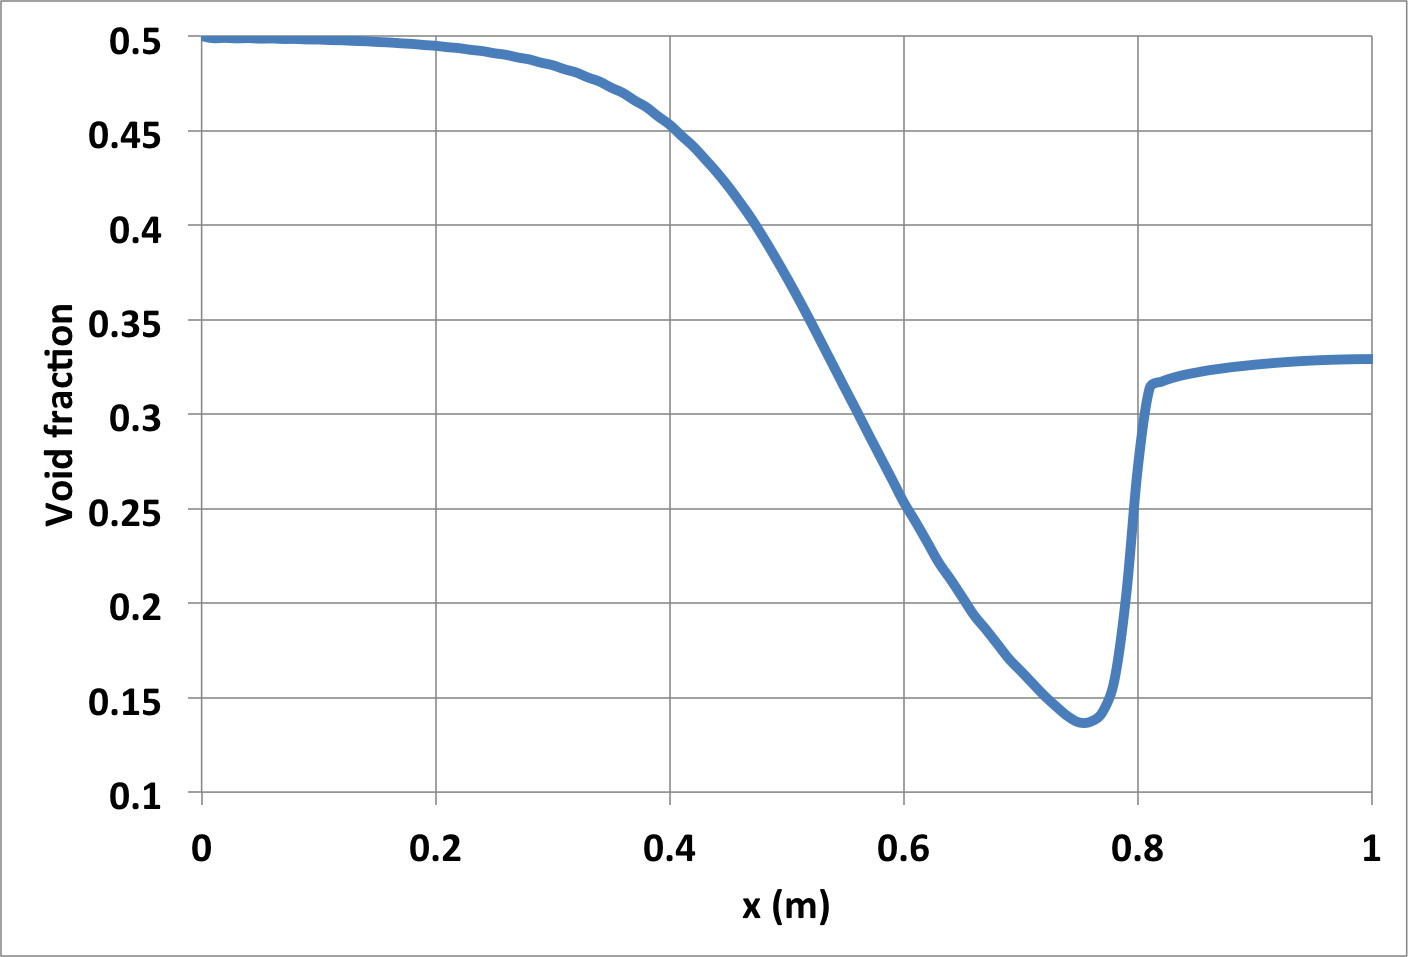
\includegraphics[width=\textwidth]{Sevan_vf.png}
%                \caption{Density.}
        \end{subfigure}
         \begin{subfigure}[b]{0.4\textwidth}
                \centering
                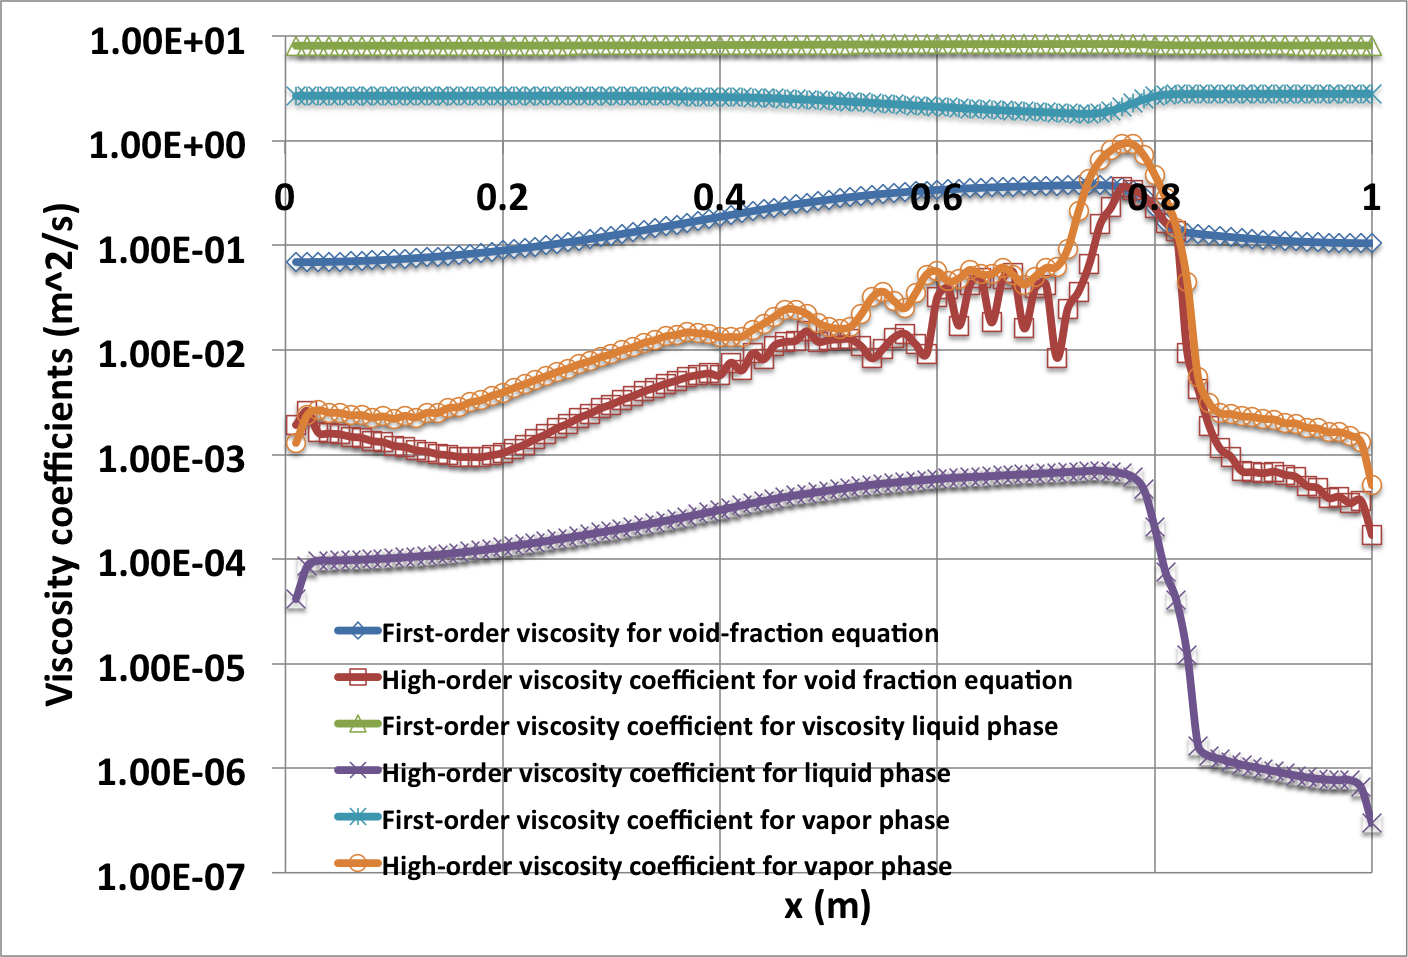
\includegraphics[width=\textwidth]{Sevan_viscosity.png}
%                \caption{Viscosity coefficients.}
        \end{subfigure}
        \caption{Steady-state numerical solution with $100$ cells, linear polynomials and BDF2.}
        \end{figure}
\end{frame}
%************************************************
\subsubsection{Conclusions: the multi-D seven-equation model.}
\begin{frame}{Conclusions: the multi-D seven-equation model.}
\begin{block}{What we have done so far:}
\begin{itemize}
\setlength{\itemsep}{15pt}
\item Derived the dissipative terms using the entropy minimum principle $\rightarrow$ valid for any equation of state under the same assumptions as for Euler equations.
\item Derived a definition for the viscosity coefficients: $\mu$, $\kappa$ and $\beta$.
\item Performed tests with a $1$-D nozzle.
\end{itemize}
\end{block}
\begin{block}{What is left to do:}
\begin{itemize}
\setlength{\itemsep}{15pt}
\item Perform some more tests in $1$-D: include mass and heat transfer between phases \cite{SEM}.
\item Tests in $2$-D.
\end{itemize}
\end{block}
\end{frame}
%************************************************
%************************************************
%************************************************
\section{A Multi-Physics Example: application of the entropy viscosity method to the $1$-D grey Radiation-Hydrodynamic equations (RHD).}
\begin{frame}
\begin{center}
\LARGE{A Multi-Physics Example: application of the entropy viscosity method to the $1$-D grey Radiation-Hydrodynamic equations (RHD).}
\end{center}
\end{frame}
%************************************************
\subsection{The $1$-D grey Radiation-Hydrodynamic equations (RHD).}
\begin{frame}{The $1$-D grey Radiation-Hydrodynamic equations (RHD):}
\begin{block}{RHD system of equations:}
\begin{equation}
\left\{
\begin{array}{lll}
\partial_t \left( \rho \right) + \partial_x\left( \rho u \right) = 0 \\
\partial_t \left( \rho u\right) + \partial_x \left(\rho u^2 + P  \right) = {\color{blue}-\partial_x \left(\frac{\epsilon}{3}\right)} \\
\partial_t \left( \rho E\right) + \partial_x \left[ u \left( \rho E + P \right) \right] = {\color{blue}-\frac{u}{3} \partial_x \epsilon - \sigma_a c \left( a T^4 - \epsilon \right)} \\
{\color{magenta}\partial_t \epsilon + \frac{4}{3} \partial_x \left( u \epsilon \right) = \frac{u}{3} \partial_x \epsilon + \partial_x \left( \frac{c}{3 \sigma_t} \partial_x \epsilon \right) + \sigma_a c \left( a T^4 - \epsilon \right)}
\end{array}
\right. 
\nonumber
\end{equation}
\end{block}
\begin{block}{A few remarks:}
\begin{itemize}
\setlength{\itemsep}{10pt}
\item The total energy (material+radiation energy density) is conserved.
\item The relaxation term $ \sigma_a c \left( a T^4 - \epsilon \right)$ behaves like a diffusion term when $\sigma_a \to \infty$ \cite{ShiJin}.
\item The above system of equations is NOT hyperbolic ???? 
\end{itemize}
\end{block}
\end{frame}
%************************************************
\subsection{Background.}
\begin{frame}{}
\begin{block}{Background:}
\begin{itemize}
\setlength{\itemsep}{15pt}
\item RHD are a wave-dominated problem.
\item They are known to develop shocks due to the nature of Euler equations.
\item Great amount of work available in the literature on how to solve RHD: approximate Riemann solver \cite{LowrieMorel, Balsara}, flux limiter \cite{EdwardsMorelKnoll}, $\cdots$
\item Have a common approach: focus on the hyperbolic part of the RHD.
\item Attempts to derive a Riemann solver accounting for the source terms.
\item Use of semi-implicit schemes because of the difference of characteristic time scale between the two physics $\rightarrow$ implicit scheme has some advantage.
\end{itemize}
\end{block}
\end{frame}
%************************************************
\begin{frame}{}
\begin{block}{Our approach:}
\begin{itemize}
\setlength{\itemsep}{10pt}
\item Consider the hyperbolic part of the system of equations (no source terms).
\item Keep in mind that the source terms may affect the entropy viscosity method and their effect will have to be studied later.
\end{itemize}
\end{block}
\begin{block}{Our hyperbolic system of equations:}
\begin{equation}
\label{eq:equation1}
\left\{
\begin{array}{lll}
\partial_t \left( \rho \right) + \partial_x\left( \rho u \right) = 0 \\
\partial_t \left( \rho u\right) + \partial_x \left(\rho u^2 + P + \frac{\epsilon}{3} \right) = 0 \\
\partial_t \left( \rho E\right) + \partial_x \left[ u \left( \rho E + P \right) \right] = 0 \\
\partial_t \epsilon + \frac{4}{3} \partial_x \left( u \epsilon \right) - \frac{u}{3} \partial_x \epsilon = 0
\end{array}
\right. 
\nonumber
\end{equation}
Eigenvalues: $\lambda_1 = u - c$, $\lambda_{2,3} = u$ and $\lambda_4 = u + c$ where $c$ is the speed of sound defined as:
\begin{equation}
c^2 =  \underbrace{P_{\rho} + \frac{P}{\rho^2}P_e}_{c^2_{\text{Euler}}} + \underbrace{ \frac{4 \epsilon}{9\rho}}_{c^2_{\text{rad}}} \nonumber
\end{equation}
\end{block}
\end{frame}
%************************************************
\subsection{Proposal.}
\begin{frame}
\begin{block}{Proposal: theoretical approach (1/2) {\color{magenta}NEW}.}
\begin{enumerate}
\setlength{\itemsep}{15pt}
\item Derive the dissipative terms using the modified system of equations (no source term). 
The entropy $s$ is assumed to be a function of three variables: the material density $\rho$ and internal energy $e$, and the radiation density energy $\epsilon$.
\item Define the viscosity coefficient(s).
\end{enumerate}
\end{block}
\begin{block}{Proposal: manufactured solutions and $1$-D results (2/2) {\color{magenta}NEW}.}
\begin{enumerate}
\setlength{\itemsep}{15pt}
\item Study the effect of the source terms, $\partial_x \left( \frac{c}{3 \sigma_t} \partial_x \epsilon \right)$ and $\sigma_a c \left( a T^4 - \epsilon \right)$, on the entropy viscosity method using the method of manufactured solutions, and show high-order convergence.
\item Perform $1$-D tests for different Mach numbers: Mach$=1.05$, $1.2$, $2$, $5$, and $50$. Semi-analytical solutions are available.
\end{enumerate}
\end{block}
\end{frame}
%************************************************
\subsection{Numerical results.}
\begin{frame}{Numerical results: Mach $1.05$.}
\begin{figure}[H]
        \centering
        \begin{subfigure}[b]{0.4\textwidth}
                \centering
                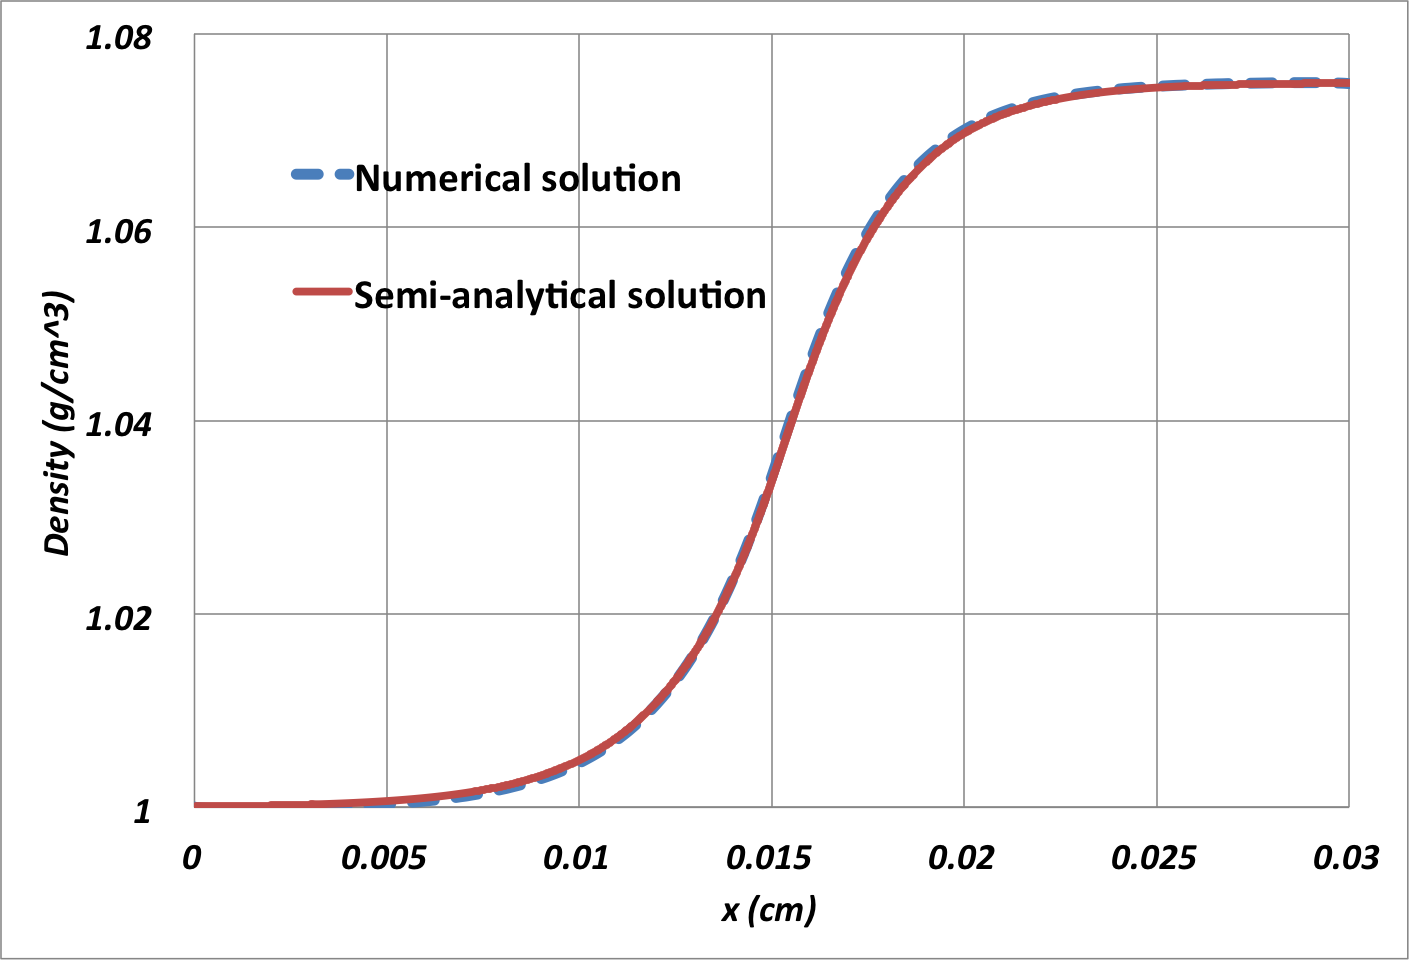
\includegraphics[width=\textwidth]{Mach1p05Density.png}
%                \caption{Pressure}
        \end{subfigure}%
        ~ %add desired spacing between images, e. g. ~, \quad, \qquad etc. 
          %(or a blank line to force the subfigure onto a new line)
        \begin{subfigure}[b]{0.4\textwidth}
                \centering
                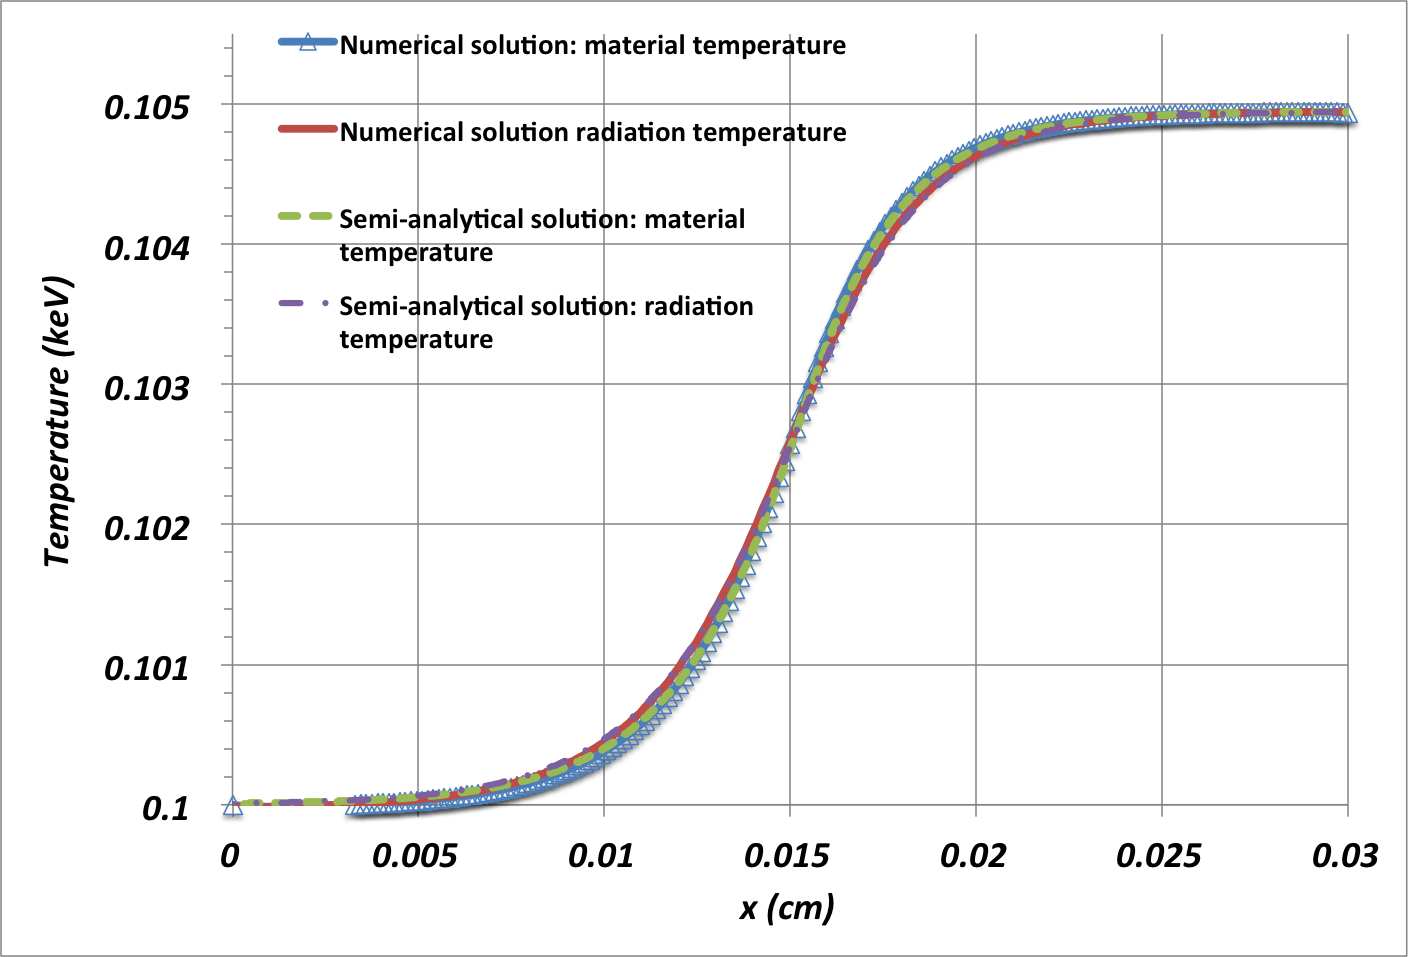
\includegraphics[width=\textwidth]{Mach1p05Temperature.png}
%                \caption{Velocity.}
        \end{subfigure}
         %add desired spacing between images, e. g. ~, \quad, \qquad etc. 
          %(or a blank line to force the subfigure onto a new line)
        \begin{subfigure}[b]{0.4\textwidth}
                \centering
                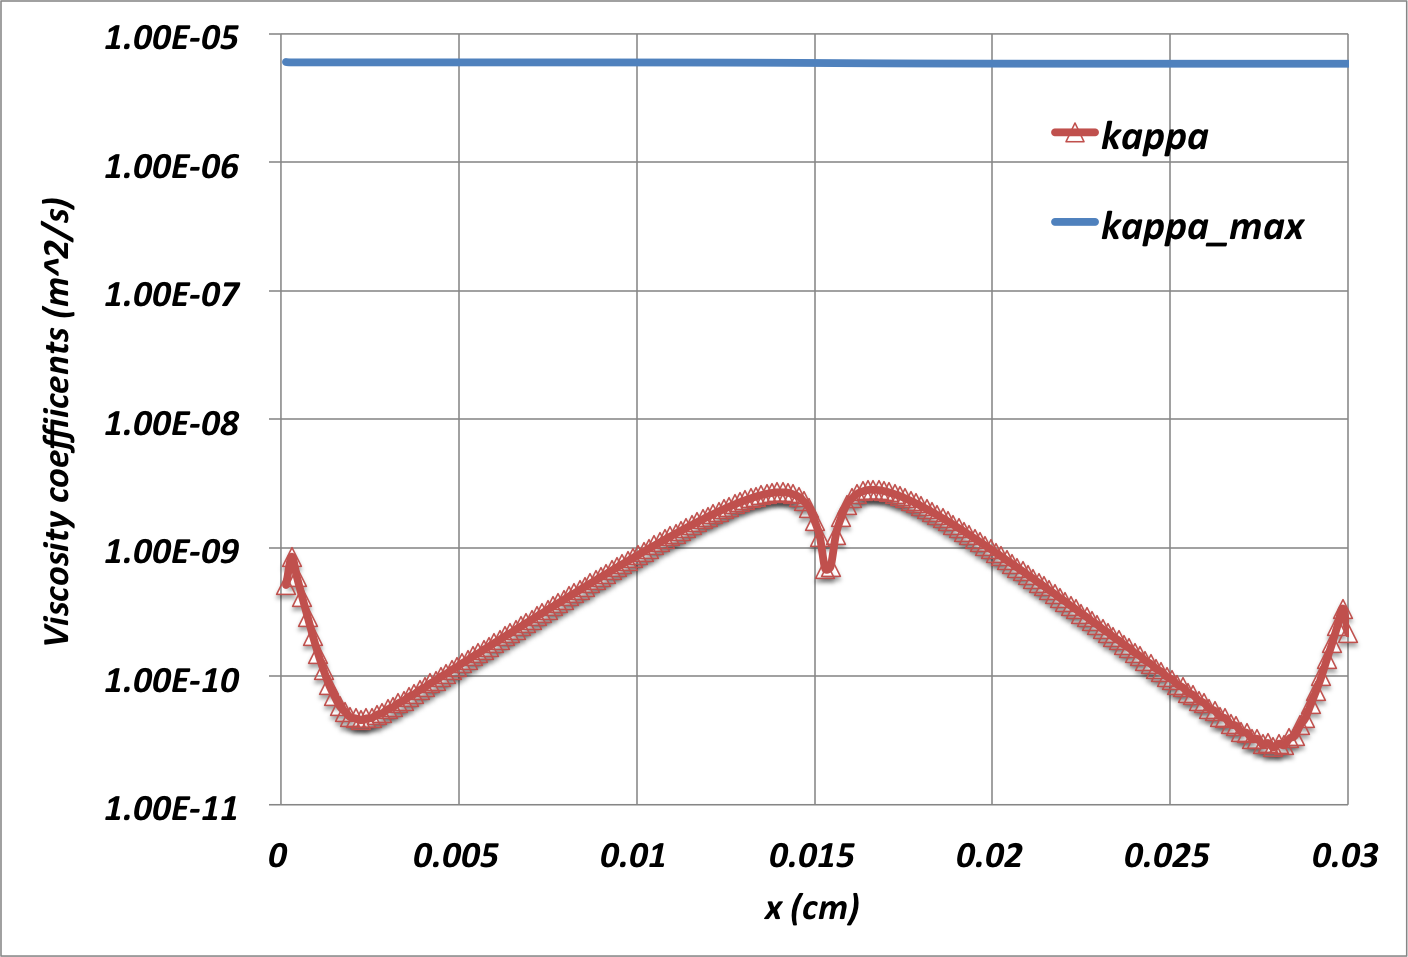
\includegraphics[width=\textwidth]{Mach1p05Viscosity.png}
%                \caption{Density.}
        \end{subfigure}
        \caption{Steady-state numerical solution with $500$ cells, linear polynomials and BDF2.}
        \end{figure}
\end{frame}
%************************************************
\begin{frame}{Numerical results: Mach $5$.}
\begin{figure}[H]
        \centering
        \begin{subfigure}[b]{0.4\textwidth}
                \centering
                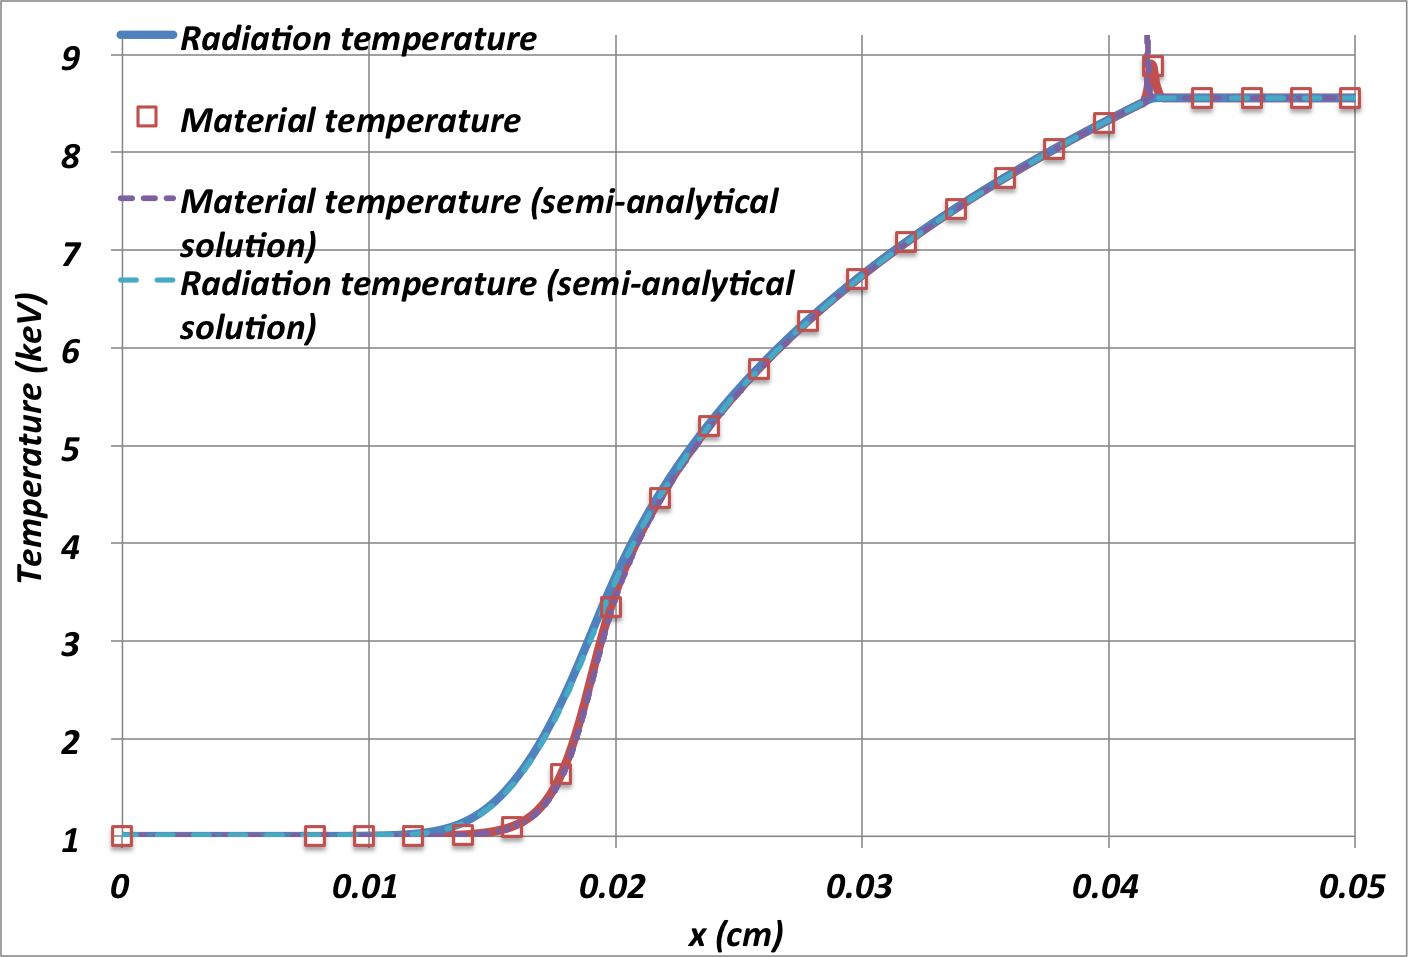
\includegraphics[width=\textwidth]{Mach5Temperature.png}
%                \caption{Pressure}
        \end{subfigure}%
        ~ %add desired spacing between images, e. g. ~, \quad, \qquad etc. 
          %(or a blank line to force the subfigure onto a new line)
        \begin{subfigure}[b]{0.4\textwidth}
                \centering
                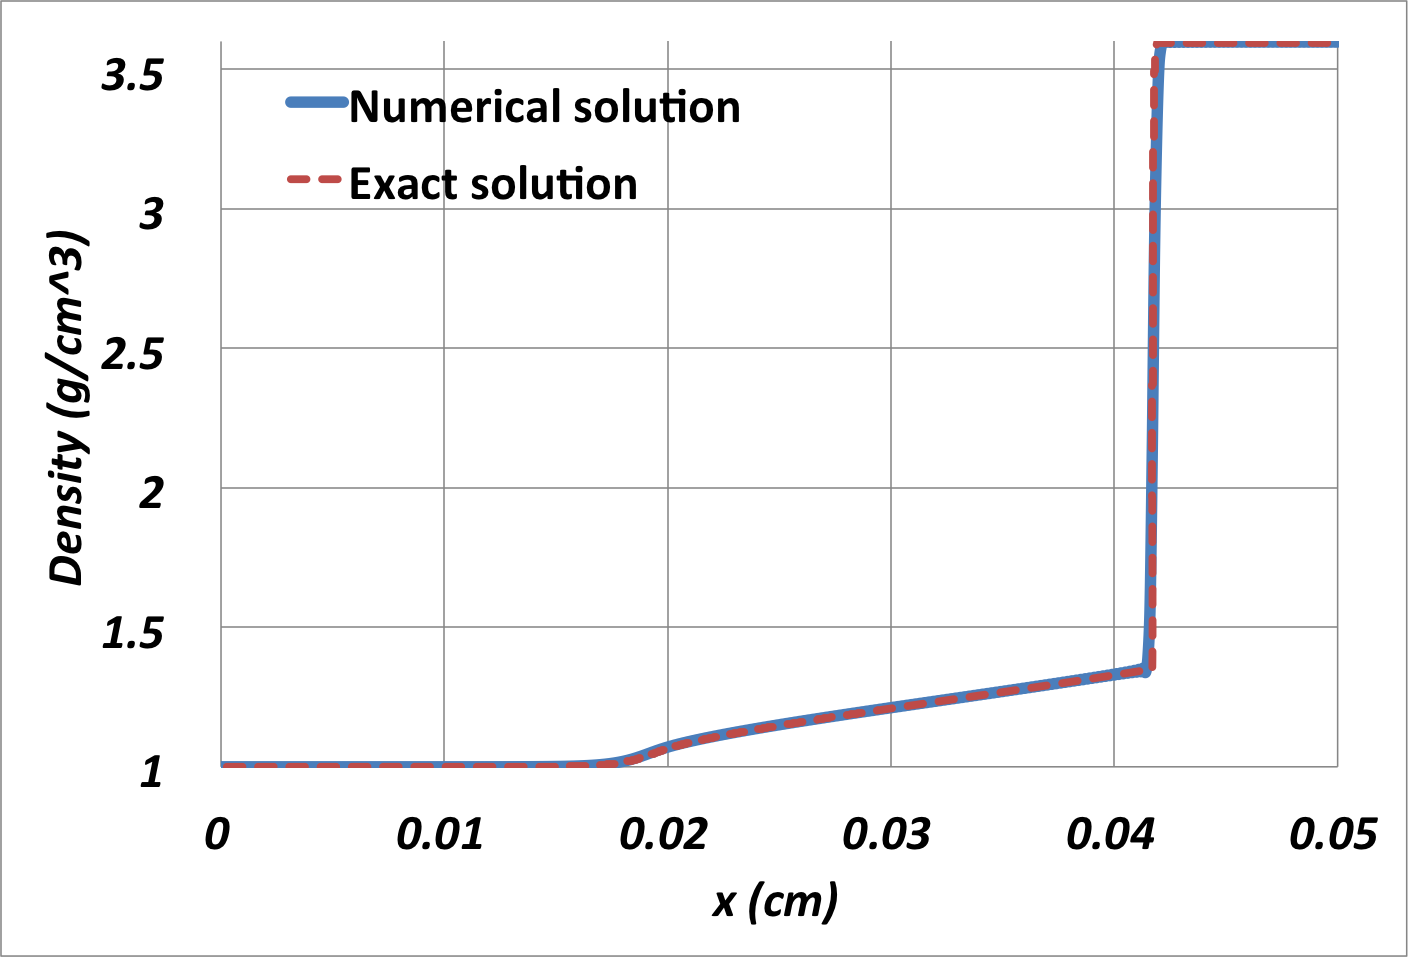
\includegraphics[width=\textwidth]{Mach5Density.png}
%                \caption{Velocity.}
        \end{subfigure}
         %add desired spacing between images, e. g. ~, \quad, \qquad etc. 
          %(or a blank line to force the subfigure onto a new line)
        \begin{subfigure}[b]{0.4\textwidth}
                \centering
                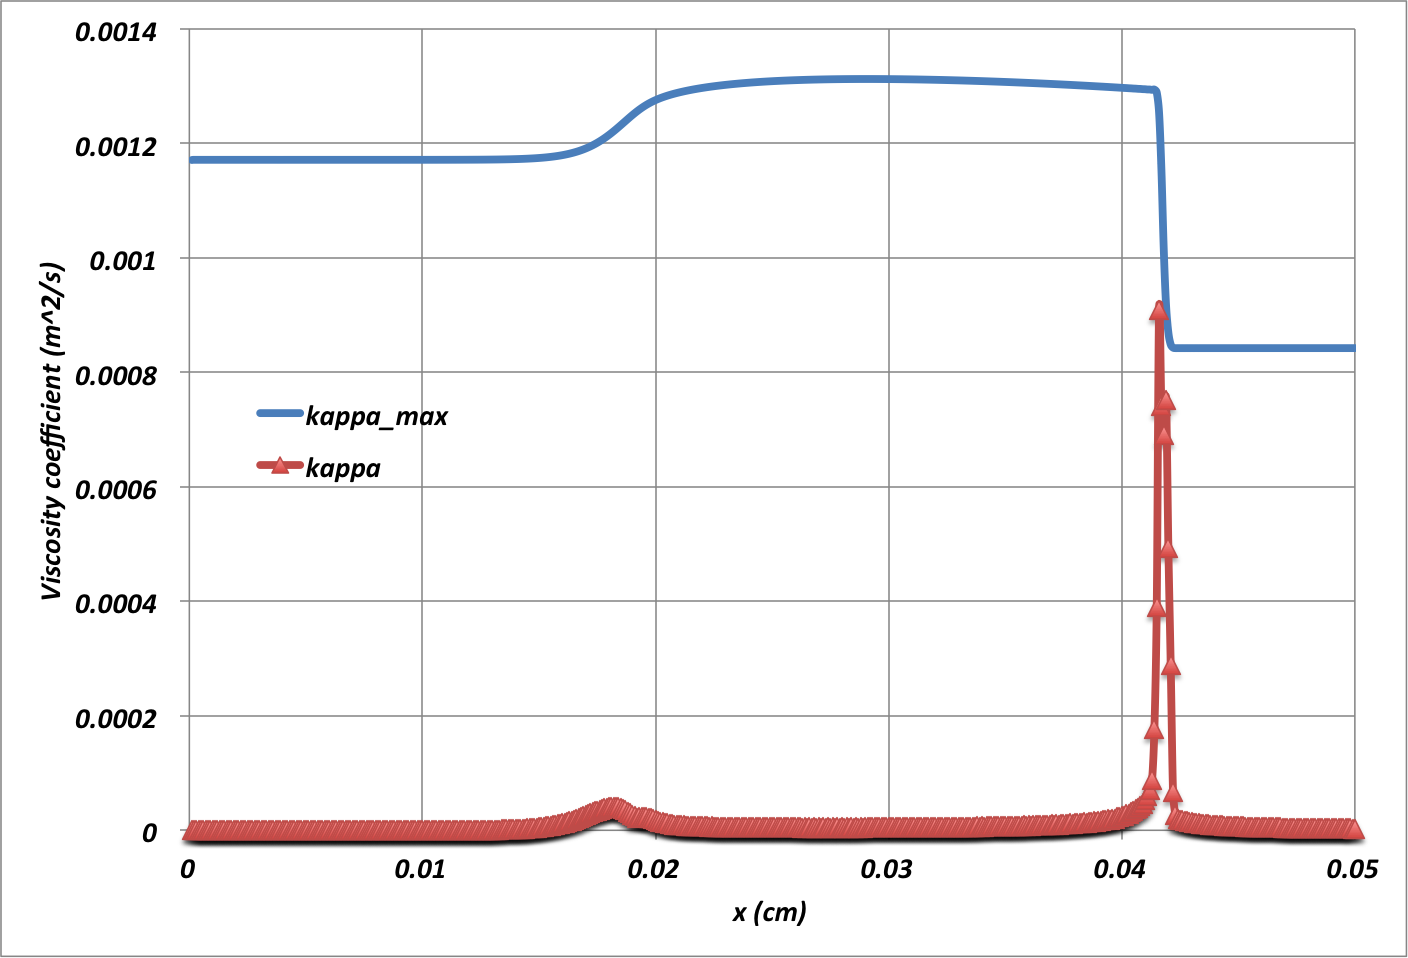
\includegraphics[width=\textwidth]{Mach5Viscosity.png}
%                \caption{Density.}
        \end{subfigure}
        \caption{Steady-state numerical solution with $500$ cells, linear polynomials and BDF2.}
        \end{figure}
\end{frame}
%************************************************
\subsection{Conclusions: RHD}
\begin{frame}
\begin{block}{Conclusions: RHD.}
\begin{itemize}
\setlength{\itemsep}{15pt}
\item The entropy viscosity method was successfully applied to the $1$-D RHD.
\item $1$-D numerical results show good agreement with semi-analytical solutions.
\item Demonstrated high-order accuracy and correct behavior in the equilibrium diffusion limit.
\end{itemize}
\end{block}
\begin{block}{General conclusions:}
\begin{itemize}
\setlength{\itemsep}{15pt}
\item The method can be applied with any equation of state with a convex entropy.
\item The method is simple to implement and the viscosity coefficient is computed on the fly.
\end{itemize}
\end{block}
\end{frame}
%************************************************
\begin{frame}{}
\begin{center}
\LARGE{\textbf{QUESTIONS/COMMENTS ?}}
\end{center}
\end{frame}
%************************************************
%************************************************
%************************************************
%************************************************
%************************************************
%************************************************
%************************************************
%************************************************
\begin{frame}[allowframebreaks]
\bibliographystyle{apalike}
\bibliography{Biblio-Database}
\begin{thebibliography}{47}
  
  \bibitem{jlg1}
  {\em Entropy viscosity method for nonlinear conservation laws}, 
  Jean-Luc Guermond, R. Pasquetti, B. Popov, J. Comput. Phys., 230 (2011) 4248-4267.
  
  \bibitem{jlg2}
  {\em Entropy Viscosity Method for High-Order Approximations of Conservation Laws}, 
  J-L. Guermond, R. Pasquetti, 
  Lecture Notes in Computational Science and Engineering, Springer, Volume 76, (2011) 411-418.

 \bibitem{jlg3}
 \emph{Entropy-based nonlinear viscosity for Fourrier approximations of conservation laws}, 
 J.-L. Guermond, R. Pasquetti, C.R. Math. Acad. Sci. Paris 346 (2008) 801�806.

  \bibitem{Neumann}
  \emph{A method for the numerical calculation of hydrodynamic shocks}, 
  J. von Neumann, R.D. Richtmyer, J. Appl. Phys. 21 (1950) 232�237
  
  \bibitem{Balsara}
  \emph{An Analysis of the Hyperbolic Nature of the Equations of Radiation Hydrodynamics},
  Dinshaw S. Balsara, J. Quant. Spectrosc. Radiat. Transfer, Vol. 61, No. 5, pp. 617-627, 1999.
  
  \bibitem{LowrieMorelHittinger}
  \emph{The coupling of radiation and hydrodynamics},
  Lowrie RB, Morel JE, Hittinger JA, 521 (1), 432-50 (1999).

  \bibitem{FluxLimiter1}
  \emph{Advanced numerical approximation of nonlinear hyperbolic equations}, 
  B. Cockburn, C. Johnson, C. Shu, E. Tadmor, Lecture Notes in Mathematics, vol. 1697, Springer, 1998.
  
  \bibitem{FluxLimiter2}
  \emph{Discontinuous Galerkin methods: theory, computation and applications}, 
  B. Cockburn, G. Karniadakis, C. Shu, Lecture Notes in Computer Science and Engineering, vol. 11, Springer, 2000.
  
  \bibitem{FluxLimiter3}
  \emph{The local discontinuous Galerkin method for time- dependent convection-diffusion systems}, 
  B. Cockburn, C. Shu, SIAM J. Numer. Anal. 35 (1998) 2440�2463.
  
\bibitem{FluxLimiter4}
\emph{New non-oscillatory central schemes on unstructured triangulations for hyperbolic systems of conservation laws}, 
I. Christov, B. Popov, J. Comput. Phys. 227 (11) (2008) 5736�5757.

\bibitem{SUPG}
\emph{Streamline upwind/Petrov-Galerkin formulations for convection dominated flows with particular emphasis on the incompressible Navier-Stokes equations},
A.N. Brooks, T.J.R. Hughes, Comput. Meths. Appl. Mech. Engrg., 32 (1982), pp. 199�259.

\bibitem{EdwardsMorelKnoll}
 \emph{Nonlinear variants of the TR$-$BDF$2$ method for thermal radiative diffusion},
 Jarrods D. Edwards, Jim E. Morel, Dana A. Knoll, Journal of Computational Physics, 230 (2011), 1198-1214.
 
  \bibitem{Toro}
  \emph{Riemann Solvers and numerical methods for fluid dynamics.}
  E.F. Toro, $2^{nd}$ Edition, Springer.  
  
  \bibitem{Reisner}
  \emph{A space-time smooth artificial viscosity method for nonlinear conservation laws}
  Reisner J., Serencsa J. and Shkoller S., Journal of Computational Physics 235 (2013) 912-933.
    
  \bibitem{valentin}
  \emph{Implementation of the entropy viscosity method with the discontinuous Galerkin method},
  Valentin Zingan, Jean-Luc Guermond, Jim Morel, Bojan Popov, Volume 253, 1 January 2013, Pages 479-490
    
  \bibitem{LowrieMorel}
  \emph{Issues with high-resolution Godunov methods for radiation hydrodynamics},
  R.B. Lowrie, J.E. Morel, Journal of Quantitative Spectroscopy \& Radiative Transfer, 69, 475-489 (2001).

\bibitem{EdwardsMorelLowrie}
\emph{Second-Order Discretization in Space and Time for Radiation Hydrodynamics},
Jarrod D. Edwards, Jim E. Morel, Robert B. Lowrie, International Conference on Mathematics and Computational Methods Applied to Nuclear Science \& Engineering (M\&C 2013), Sun Valley, Idaho USA, May 5-9, American Nuclear Society, LaGrange Park, II (2013).
   
  \bibitem{ShiJin}
  \emph{Numerical Schemes for Hyperbolic Conservation Laws with Stiff Relaxation Terms}, 
  Shi Jin and C. David Levermore, Journal of Computational Physics, 126, 449-467 (1996).
  
  \bibitem{jlg}
  \emph{Viscous regularization of the Euler equations and entropy principles},
  Jean-Luc Guermond and Bojan Popov, under review.
  
  \bibitem{Moose}
  \emph{A parallel computational framework for coupled systems of nonlinear equations},
  D. Gaston, C. Newsman, G. Hansen and D. Lebrun-Grandie, Nucl. Eng. Design, vol 239, pp 1768-1778, 2009.
  
  \bibitem{Sodov}
  \emph{Similarity and dimensional methods in mechanics},
  Sedov LI., New York: Academic Press, 1959.
  
  \bibitem{RatTherm}
  \emph{Rational thermodynamics},
  Truesdell C. and Wang C.-C., New York, McGraw-Hill Book Company, 1969, XII. 208 S.
  
  \bibitem{IGEOS}
  \emph{A to Z of Thermodynamics},
  Perrot P., Oxford University Press (1998).
  
  \bibitem{SGEOS}
  \emph{Elaborating equation of state for a liquid and its vapor for two-phase flow models.}
  O. LeMetayer, J. Massoni, R. Saurel, International Journal of Thermal Science 43 (2004) 265-276.

  \bibitem{Lapidus_paper}
  \emph{A detached shock calculation by second order finite differences},
  Lapidus A., J. Comput. Phys., 2, 154-177.

  \bibitem{LMP}
  \emph{A simple extension to multidimensional problems of the artificial viscosity due to Lapidus},
  Lohner R., Morgan K. and Peraire J., Commun. Numer. Methods Eng., 1(14), 141-147.
      
  \bibitem{Lapidus_book}
  \emph{Finite Element Methods for Flow Problems},
  Jean Donea and Antonio Huerta, 2003,  Edition, Wiley.
  
  \bibitem{PBV_book}
  \emph{Applied CFD Techniques: an Introduction based on Finite Element Methods},
  Rainald Lohner, $2^{nd}$ Edition, Wiley.
  
  \bibitem{Roe}
  \emph{An All-Speed Roe-type scheme and its asymptotic analysis of low Mach number behavior},
  Xue-song Li, Chun-wei Gu, Journal of Computational Physics 227 (2008) 5144-5159
  
  \bibitem{LowMach1}
  \emph{On the behavior of upwind schemes in the low Mach number limit},
  Guillard H., Viozat C., Computers \& Fluids 28 (1999) 63-86.
  
  \bibitem{LowMach2}
  \emph{Preconditioned techniques in computational fluid dynamics.}
  E.Turkel, Annu. Rev. Fluid Mech. (1999) 31:385-416.  
  
  \bibitem{LowMach3}
  \emph{The solution of the compressible Euler equations at low Mach numbers using a stabilized finite element algorithm},
  J. S. Wong, D.L. Darmofal, J. Peraire, Comput. Methods Appl. Mech. Engrg. 190 (2001) 5719-5737.
  
  \bibitem{SEM}
  \emph{The discrete equation method (DEM) for fully compressible, two-phase flows in ducts of spatially varying cross-section.}
  R. Berry, R. Saurel, O. LeMetayer,
  Nuclear Engineering and Design, 240 (2010) 3797-3818.
  
  \bibitem{Riemann12}
  \emph{Comparison of several difference schemes on 1D and 2D test problems for the Euler equations}, 
  R. Liska, B. Wendroff, SIAM J. Sci. Comput. 25 (3) (2003) 995� 1017 (electronic).
  
  \bibitem{Mach3Step}
  \emph{An evaluation of several differencing methods for inviscid fluid flow problems}, 
  A.F. Emery, J. Comput. Phys. 2 (1968) 306�331.
  
  \bibitem{CompressionCorner}
  \emph{Modern Compressible Flow}, 
  Anderson, J.D. (1982), McGraw Hill Inc., New York. ASME (2006). V\&V 10-2006 Guide for Verification and Validation in Computational Solid
Mechanic.
  
  \bibitem{Hump}
  \emph{A Robust Multigrid Algorithm for the Euler Equations with Local Preconditioning and Semi-coarsening},
  D. L. Darmofal and K. Siu, Journal of Computational Physics 151, 728�756 (1999).
  
  \bibitem{Leblanc}
  \emph{Validation Test Case Suite for compressible hydrodynamics computation},
  Loubere R., Theoritical Division, T-7, Los Alamos National Laboratory (pdf version).
  
  \bibitem{ShockTEOS}
  \emph{A New Averaging Scheme for the Riemann Problem in Pure Water},
  Tze-Jang Chen, C. H. Cooke, Mathl. Comput. Modeling Vol. 25 No. 3, pp. 25-36, 1997.
\end{thebibliography}
\end{frame}
%************************************************
%************************************************
%************************************************
%************************************************
%************************************************
%************************************************
%************************************************
%************************************************
\begin{frame}{Viscous regularization for the multi-D Euler equations (with variable area):}
\begin{block}{}
\begin{eqnarray}
\left\{
\begin{array}{llll}
\partial_t \left(\rho A\right) + \div \left(\rho \vec{u} A\right) = {\color{red}\div \left(A \kappa \grad \rho \right)}  \\
\partial_t \left(\rho \vec{u} A\right) + \div \left(\rho \vec{u} \otimes \vec{u} A\right) + \grad(P A) = P \grad A + {\color{red}\div\left[ A\left( \mu \rho \grad^s \vec{u} + \vec{u} \otimes \left( \kappa \grad \rho \right) \right)\right]}   \nonumber\\
\partial_t \left(\rho E A\right) + \div \left[\vec{u}(\rho E + P)A\right] = {\color{red}\div\left[ A \left( \kappa \grad (\rho e) + \frac{||\vec{u}||^2}{2} \kappa \grad \rho + \mu \rho \vec{u} \cdot \grad^s \vec{u} \right)\right]} \\
P = eos(\rho, e) 
\end{array}
\right.
\end{eqnarray}
\end{block}
\end{frame}
%************************************************
\begin{frame}{Viscous regularization for the multi-D seven-equation model:}
\begin{equation}
\left\{
\begin{array}{lll}
\partial_t \left( \alpha_k  A\right) &+ \vec{u}_I A \grad \alpha_k = {\color{blue}A \mu_{rel} \left( P_k - P_j \right)} + {\color{red}\div \vec{l}} & \nonumber \\
\partial_t \left( \alpha_k \rho_k A \right) &+ \div \left( \alpha_k \rho_k \vec{u}_k A \right) = {\color{red}\div \vec{f}}& \nonumber \\
\partial_t \left( \alpha_k \rho_k \vec{u}_k A \right) &+ \div \left[ \alpha_k A \left( \rho_k \vec{u}_k\otimes \vec{u}_k \right) \right]  + \grad(\alpha_k A P_k) =  \nonumber \\
&\alpha_k P_k \grad A +  P_I A \grad \alpha_k +  {\color{blue}A \lambda_{rel} \left( \vec{u}_j - \vec{u}_k \right)} +{\color{red}\div \bar{g}}&\nonumber \\
\partial_t \left( \alpha_k \rho_k E_k A \right) &+ \div \left[ \alpha_k A \vec{u}_j \left( \rho_k E_k + P_k \right) \right] =& \\
 &P_I \vec{u}_I A \grad \alpha_k - {\color{blue}\mu_{rel} \bar{P_I} \left( P_k-P_j \right)} +{\color{blue}\bar{\vec{u}}_kA \lambda_{rel} \left( \vec{u}_j - \vec{u}_k \right)} + {\color{red}\div \vec{h}}& \nonumber
\end{array}
\right.
\end{equation}
\begin{equation}
\left\{
\begin{array}{lcl}
{\color{red}\vec{l}} = A {\color{magenta}\beta_k} \grad \alpha_k & & \\
{\color{red}\vec{f}} = \alpha_k A {\color{magenta}\kappa_k}  \grad \rho_k + \rho_k \vec{l}& & \\
{\color{red}\bar{g}} = \alpha_k A \rho_k {\color{magenta}\mu_k} \grad \vec{u} + \vec{u} \otimes \vec{f} & & \\
{\color{red}\vec{h}} = \alpha_k A {\color{magenta}\kappa_k} \grad(\rho_k e_k) - \frac{||\vec{u}||^2}{2} \vec{f} + \vec{u} \cdot \bar{g} + \rho_k e_k \vec{l} & &
\end{array}
\right.
\nonumber
\end{equation}
Entropy equation:
\begin{eqnarray}
\alpha_k A \rho_k \frac{ds_k}{dt} + \left( {\color{green}\alpha_k A \rho_k \kappa_k} + {\color{red}\rho_k l_k} \right) \grad s_k - {\color{green}\div \left( \alpha_k A \rho_k \grad s_k \right)} = \nonumber \\ {\color{green}\partial_e s_k \alpha_k A \rho_k \mu_k \grad^s \vec{u} :  \grad \vec{u}}- {\color{green}X_k \Sigma_k X_k^t} + {\color{blue}Q}
\nonumber
\end{eqnarray}
\end{frame}
%************************************************
\begin{frame}{$2$-D numerical results: hump.}
Isomachs for $M=0.001$ with $2352$ elements.
\begin{figure}[H]
                \centering
                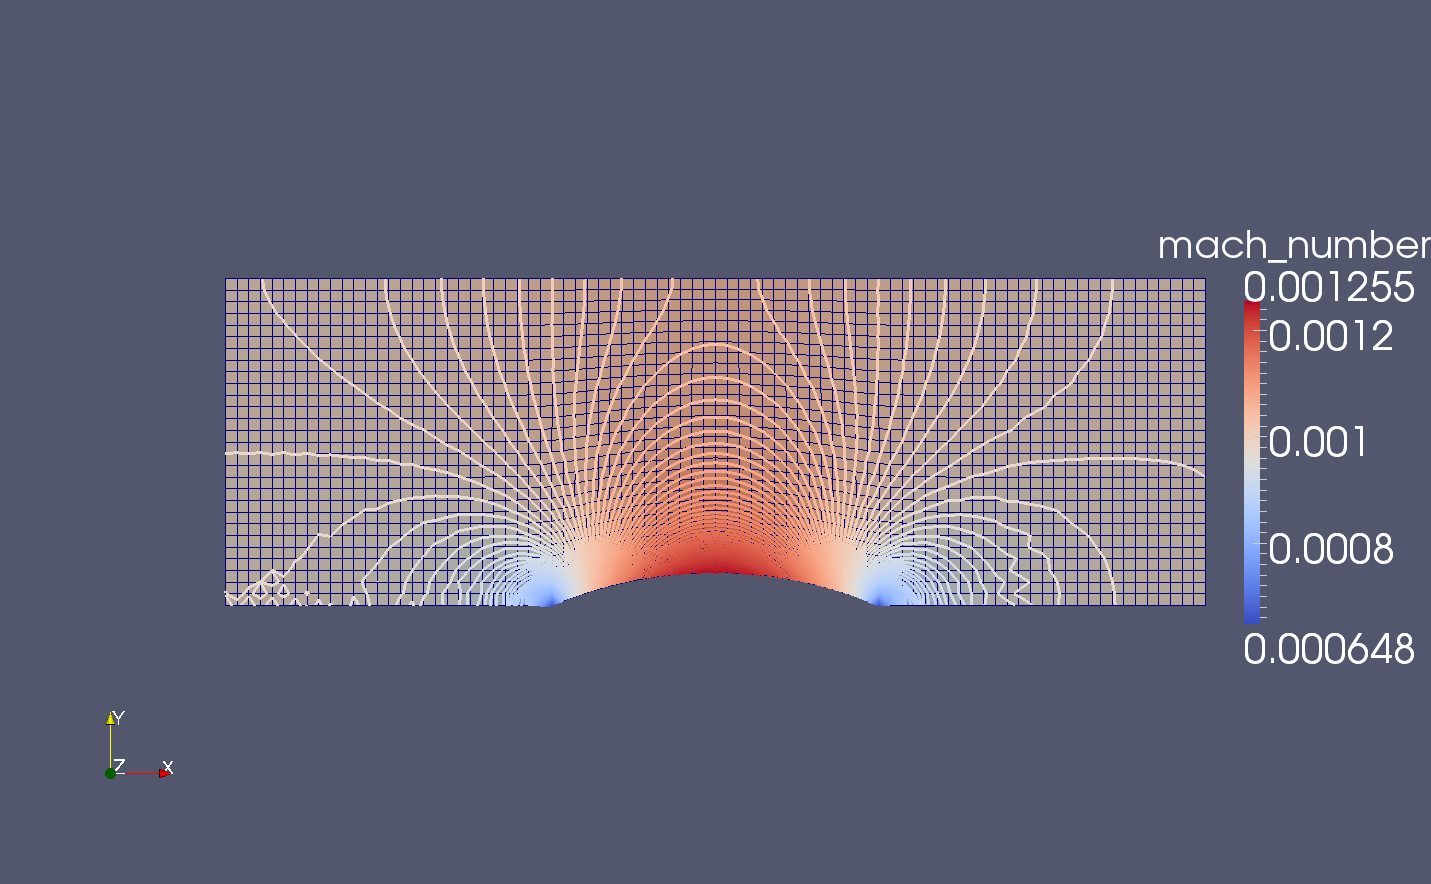
\includegraphics[width=\textwidth]{Hump2Dmach0001MachNumber.png}
\end{figure}
\end{frame}
%************************************************
\begin{frame}{$2$-D numerical results: hump.}
Viscosity for $M=0.001$ with $2352$ elements.
\begin{figure}[H]
                \centering
                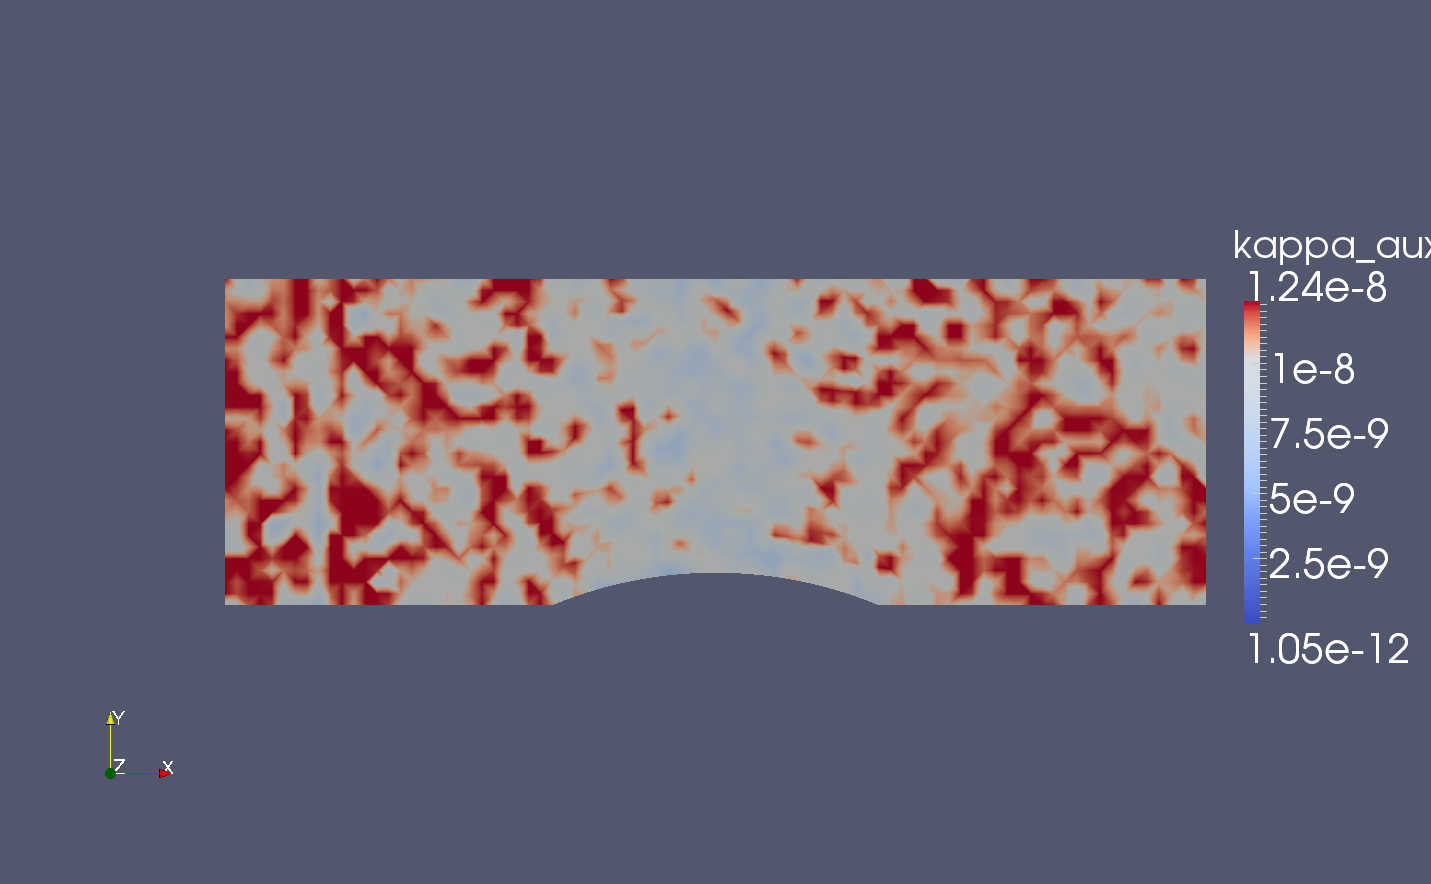
\includegraphics[width=\textwidth]{Hump2Dmach0001Viscosity.png}
\end{figure}
\end{frame}
%************************************************
\begin{frame}{$2$-D numerical results: cylinder.}
Mach number for $M_{\infty}=0.05$.
\begin{figure}[H]
                \centering
                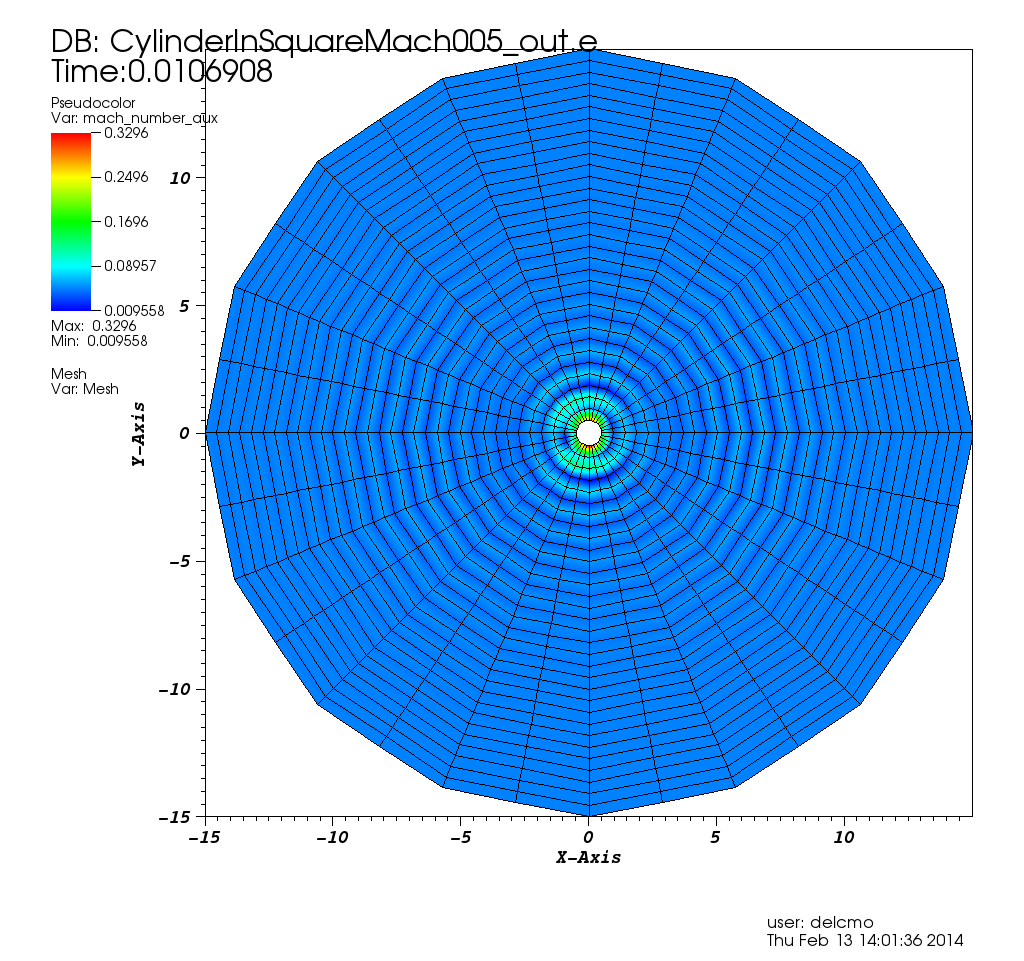
\includegraphics[scale=0.24]{visit0001.png}
\end{figure}
\end{frame}
\end{document}

